% Options for packages loaded elsewhere
% Options for packages loaded elsewhere
\PassOptionsToPackage{unicode}{hyperref}
\PassOptionsToPackage{hyphens}{url}
\PassOptionsToPackage{dvipsnames,svgnames,x11names}{xcolor}
%
\documentclass[
  10pt,
  a4paper,
  DIV=11,
  numbers=noendperiod]{scrartcl}
\usepackage{xcolor}
\usepackage[top = 2cm,bottom = 2cm,left = 2.5cm,right = 2.5cm,footskip =
20pt]{geometry}
\usepackage{amsmath,amssymb}
\setcounter{secnumdepth}{5}
\usepackage{iftex}
\ifPDFTeX
  \usepackage[T1]{fontenc}
  \usepackage[utf8]{inputenc}
  \usepackage{textcomp} % provide euro and other symbols
\else % if luatex or xetex
  \usepackage{unicode-math} % this also loads fontspec
  \defaultfontfeatures{Scale=MatchLowercase}
  \defaultfontfeatures[\rmfamily]{Ligatures=TeX,Scale=1}
\fi
\usepackage{lmodern}
\ifPDFTeX\else
  % xetex/luatex font selection
\fi
% Use upquote if available, for straight quotes in verbatim environments
\IfFileExists{upquote.sty}{\usepackage{upquote}}{}
\IfFileExists{microtype.sty}{% use microtype if available
  \usepackage[]{microtype}
  \UseMicrotypeSet[protrusion]{basicmath} % disable protrusion for tt fonts
}{}
\usepackage{setspace}
\makeatletter
\@ifundefined{KOMAClassName}{% if non-KOMA class
  \IfFileExists{parskip.sty}{%
    \usepackage{parskip}
  }{% else
    \setlength{\parindent}{0pt}
    \setlength{\parskip}{6pt plus 2pt minus 1pt}}
}{% if KOMA class
  \KOMAoptions{parskip=half}}
\makeatother
% Make \paragraph and \subparagraph free-standing
\makeatletter
\ifx\paragraph\undefined\else
  \let\oldparagraph\paragraph
  \renewcommand{\paragraph}{
    \@ifstar
      \xxxParagraphStar
      \xxxParagraphNoStar
  }
  \newcommand{\xxxParagraphStar}[1]{\oldparagraph*{#1}\mbox{}}
  \newcommand{\xxxParagraphNoStar}[1]{\oldparagraph{#1}\mbox{}}
\fi
\ifx\subparagraph\undefined\else
  \let\oldsubparagraph\subparagraph
  \renewcommand{\subparagraph}{
    \@ifstar
      \xxxSubParagraphStar
      \xxxSubParagraphNoStar
  }
  \newcommand{\xxxSubParagraphStar}[1]{\oldsubparagraph*{#1}\mbox{}}
  \newcommand{\xxxSubParagraphNoStar}[1]{\oldsubparagraph{#1}\mbox{}}
\fi
\makeatother


\usepackage{longtable,booktabs,array}
\newcounter{none} % for unnumbered tables
\usepackage{calc} % for calculating minipage widths
% Correct order of tables after \paragraph or \subparagraph
\usepackage{etoolbox}
\makeatletter
\patchcmd\longtable{\par}{\if@noskipsec\mbox{}\fi\par}{}{}
\makeatother
% Allow footnotes in longtable head/foot
\IfFileExists{footnotehyper.sty}{\usepackage{footnotehyper}}{\usepackage{footnote}}
\makesavenoteenv{longtable}
\usepackage{graphicx}
\makeatletter
\newsavebox\pandoc@box
\newcommand*\pandocbounded[1]{% scales image to fit in text height/width
  \sbox\pandoc@box{#1}%
  \Gscale@div\@tempa{\textheight}{\dimexpr\ht\pandoc@box+\dp\pandoc@box\relax}%
  \Gscale@div\@tempb{\linewidth}{\wd\pandoc@box}%
  \ifdim\@tempb\p@<\@tempa\p@\let\@tempa\@tempb\fi% select the smaller of both
  \ifdim\@tempa\p@<\p@\scalebox{\@tempa}{\usebox\pandoc@box}%
  \else\usebox{\pandoc@box}%
  \fi%
}
% Set default figure placement to htbp
\def\fps@figure{htbp}
\makeatother


% definitions for citeproc citations
\NewDocumentCommand\citeproctext{}{}
\NewDocumentCommand\citeproc{mm}{%
  \begingroup\def\citeproctext{#2}\cite{#1}\endgroup}
\makeatletter
 % allow citations to break across lines
 \let\@cite@ofmt\@firstofone
 % avoid brackets around text for \cite:
 \def\@biblabel#1{}
 \def\@cite#1#2{{#1\if@tempswa , #2\fi}}
\makeatother
\newlength{\cslhangindent}
\setlength{\cslhangindent}{1.5em}
\newlength{\csllabelwidth}
\setlength{\csllabelwidth}{3em}
\newenvironment{CSLReferences}[2] % #1 hanging-indent, #2 entry-spacing
 {\begin{list}{}{%
  \setlength{\itemindent}{0pt}
  \setlength{\leftmargin}{0pt}
  \setlength{\parsep}{0pt}
  % turn on hanging indent if param 1 is 1
  \ifodd #1
   \setlength{\leftmargin}{\cslhangindent}
   \setlength{\itemindent}{-1\cslhangindent}
  \fi
  % set entry spacing
  \setlength{\itemsep}{#2\baselineskip}}}
 {\end{list}}
\usepackage{calc}
\newcommand{\CSLBlock}[1]{\hfill\break\parbox[t]{\linewidth}{\strut\ignorespaces#1\strut}}
\newcommand{\CSLLeftMargin}[1]{\parbox[t]{\csllabelwidth}{\strut#1\strut}}
\newcommand{\CSLRightInline}[1]{\parbox[t]{\linewidth - \csllabelwidth}{\strut#1\strut}}
\newcommand{\CSLIndent}[1]{\hspace{\cslhangindent}#1}



\setlength{\emergencystretch}{3em} % prevent overfull lines

\providecommand{\tightlist}{%
  \setlength{\itemsep}{0pt}\setlength{\parskip}{0pt}}



 


\usepackage{setspace}
\setlength{\parindent}{15pt}
\usepackage[font=scriptsize]{caption}
\KOMAoption{captions}{tableheading}
\makeatletter
\@ifpackageloaded{caption}{}{\usepackage{caption}}
\AtBeginDocument{%
\ifdefined\contentsname
  \renewcommand*\contentsname{Table of contents}
\else
  \newcommand\contentsname{Table of contents}
\fi
\ifdefined\listfigurename
  \renewcommand*\listfigurename{List of Figures}
\else
  \newcommand\listfigurename{List of Figures}
\fi
\ifdefined\listtablename
  \renewcommand*\listtablename{List of Tables}
\else
  \newcommand\listtablename{List of Tables}
\fi
\ifdefined\figurename
  \renewcommand*\figurename{Figure}
\else
  \newcommand\figurename{Figure}
\fi
\ifdefined\tablename
  \renewcommand*\tablename{Table}
\else
  \newcommand\tablename{Table}
\fi
}
\@ifpackageloaded{float}{}{\usepackage{float}}
\floatstyle{ruled}
\@ifundefined{c@chapter}{\newfloat{codelisting}{h}{lop}}{\newfloat{codelisting}{h}{lop}[chapter]}
\floatname{codelisting}{Listing}
\newcommand*\listoflistings{\listof{codelisting}{List of Listings}}
\makeatother
\makeatletter
\makeatother
\makeatletter
\@ifpackageloaded{caption}{}{\usepackage{caption}}
\@ifpackageloaded{subcaption}{}{\usepackage{subcaption}}
\makeatother
\usepackage{bookmark}
\IfFileExists{xurl.sty}{\usepackage{xurl}}{} % add URL line breaks if available
\urlstyle{same}
\hypersetup{
  pdftitle={Penalized for Faith: Who Drives the Muslim Penalty?},
  pdfauthor={Tristan Muno; Vera Okisheva; Raphael Klöckner},
  colorlinks=true,
  linkcolor={blue},
  filecolor={Maroon},
  citecolor={Blue},
  urlcolor={Blue},
  pdfcreator={LaTeX via pandoc}}


\title{Penalized for Faith: Who Drives the Muslim Penalty?}
\usepackage{etoolbox}
\makeatletter
\providecommand{\subtitle}[1]{% add subtitle to \maketitle
  \apptocmd{\@title}{\par {\large #1 \par}}{}{}
}
\makeatother
\subtitle{Treatment-Effect Heterogeneity in European Conjoint Behavioral
Games}
\author{Tristan Muno \and Vera Okisheva \and Raphael Klöckner}
\date{June 11, 2026}
\begin{document}
\maketitle
\begin{abstract}
Conjoint experiments across Europe consistently reveal a Muslim penalty:
profiles displayed as Muslim receive systematically fewer resources than
otherwise comparable profiles. We move beyond this average and ask who
drives the penalty. Reanalyzing dictator and trust games embedded in a
conjoint experiment across 25 European countries, we treat the Muslim
attribute as a binary treatment and estimate conditional average
treatment effects with Causal Forests. The penalty is negative in
essentially every subgroup we examine. The other attributes of the
displayed profile moderate it only weakly. Respondent characteristics
matter more. Evaluations of the European Union form the strongest and
most coherent gradient, yet even the most pro-European respondents
retain a clear penalty. Anti-Muslim bias in Europe emerges as
politically structured rather than idiosyncratic, attenuated but nowhere
undone.
\end{abstract}


\setstretch{1}
\section{Introduction}\label{sec-introduction}

Experimental research has documented a robust Muslim penalty across
European societies (\citeproc{ref-helbling2012islamophobia}{Helbling
2012}). Individuals identified as Muslim receive less help in everyday
encounters (\citeproc{ref-choi2023hijab}{Choi et al. 2023}), are less
welcome as labor migrants and refugees
(\citeproc{ref-helbling2022muslim}{Helbling et al. 2022}), and elicit
weaker opposition to their persecution abroad
(\citeproc{ref-findor2025anti}{Findor et al. 2025}). Yet establishing
the existence of this penalty, that is the systematic disadvantage
incurred by individuals identified as Muslim, is only the starting point
for a substantive understanding of the phenomenon. The more demanding
questions concern who discriminates, against whom, and under which
conditions.

Against this background, this paper revisits a large-scale conjoint
survey experiment conducted across 25 European Union member states by
Hahm et al. (\citeproc{ref-hahm2024divided}{2024}). Using a combination
of dictator and trust games alongside a conjoint design, they estimate
the relative strength of multiple social divides. Their main finding is
the dominance of the partisan divide, but religion emerges as the second
strongest divide in their analysis. Whenever Muslim identity is
experimentally signaled, respondents' allocation decisions reveal a
systematic penalty relative to otherwise comparable non-Muslim profiles
(Table~\ref{tbl-diff-in-means}). What these averages do not reveal is
whether and how the magnitude of the penalty varies with the other
attributes attached to Muslim profiles, with the characteristics and
political orientations of respondents, or with the interaction between
the two.

This paper takes that heterogeneity as its central object of inquiry.
Treating the Muslim penalty as the primary quantity of interest, it
shifts from the average effects conventionally reported in conjoint
analyses toward a conditional average treatment effect logic and
distinguishes two sources of variation
(\citeproc{ref-robinson2024detect}{Robinson and Duch 2024}). The first
concerns whether the remaining attributes of the displayed Muslim
profile, such as class, nationality, or EU stance, moderate the
magnitude of the penalty. The second, and substantively more
consequential, concerns whether individual-level characteristics of
respondents, in particular their populist predispositions and their
orientations toward European integration, account for who discriminates
more strongly. The literature gives strong reasons to expect that the
penalty is conditional rather than uniform. Hostility toward Muslims is
driven less by nominal religious affiliation than by perceived
religiosity (\citeproc{ref-helbling2020islamophobia}{Helbling and
Traunmüller 2020}; \citeproc{ref-helbling2022muslim}{Helbling et al.
2022}). Discriminatory behavior responds to signals about a Muslim
target's values and differs with the discriminator's own gender and
ideology (\citeproc{ref-choi2023hijab}{Choi et al. 2023}). And
anti-Muslim bias in policy attitudes appears only among respondents
holding negative or neutral prior views of Muslims, varying more with
individual attitudes than with country context
(\citeproc{ref-findor2025anti}{Findor et al. 2025}). What is missing is
a systematic account of this variation within a single behavioral
design.

We reanalyze roughly 84,600 allocation decisions per game with Causal
Forests (CF), treating the Muslim attribute as a binary treatment and
recovering conditional effects across pre-specified profile-level and
respondent-level moderators. A hierarchical Bayesian Causal Forest (BCF)
serves as a robustness check. Three findings stand out. First, the
penalty is negative in essentially every subgroup we examine. Second,
the other profile attributes moderate it only weakly, with displayed
partisanship the main exception. Third, respondent characteristics
matter more, and evaluations of the European Union form the strongest
and most coherent gradient. Respondents hostile to the Union penalize
Muslim profiles substantially more, yet even the most pro-European
retain a clear penalty.

These results promote a more nuanced understanding of anti-Muslim
discrimination in Europe. The variation in penalties tracks the
cosmopolitan--populist divide that defines contemporary European
politics, suggesting a bias that is less an isolated individual
disposition than a politically structured phenomenon. Understanding the
conditions that amplify this bias is crucial for grasping the mechanisms
that sustain it and the potential avenues for its mitigation.

{

\begin{longtable}[]{@{}
  >{\raggedright\arraybackslash}p{(\linewidth - 8\tabcolsep) * \real{0.1795}}
  >{\raggedright\arraybackslash}p{(\linewidth - 8\tabcolsep) * \real{0.2436}}
  >{\raggedright\arraybackslash}p{(\linewidth - 8\tabcolsep) * \real{0.2436}}
  >{\raggedright\arraybackslash}p{(\linewidth - 8\tabcolsep) * \real{0.1026}}
  >{\raggedright\arraybackslash}p{(\linewidth - 8\tabcolsep) * \real{0.2051}}@{}}

\caption{\label{tbl-diff-in-means}Mean tokens allocated to a profile by
the Muslim label, by game. The outcome is the number of tokens the
respondent allocates to the displayed profile. Profiles labelled Muslim
are contrasted against all other religions pooled. The first two columns
show group means with 95\% confidence intervals in brackets. The SATE
column reports the sample average treatment effect of the Muslim label,
estimated by a per-game Welch two-sample difference-in-means t-test,
with its 95\% confidence interval alongside. The test is intentionally
simple and descriptive. Respondent clustering is left to the
heterogeneity models.}

\tabularnewline

\toprule\noalign{}
\begin{minipage}[b]{\linewidth}\raggedright
Game
\end{minipage} & \begin{minipage}[b]{\linewidth}\raggedright
Muslim
\end{minipage} & \begin{minipage}[b]{\linewidth}\raggedright
Non-Muslim
\end{minipage} & \begin{minipage}[b]{\linewidth}\raggedright
SATE
\end{minipage} & \begin{minipage}[b]{\linewidth}\raggedright
95\% CI
\end{minipage} \\
\midrule\noalign{}
\endhead
\bottomrule\noalign{}
\endlastfoot
Dictator game & 2.80 {[}2.77, 2.84{]} & 3.37 {[}3.36, 3.39{]} & -0.57 &
{[}-0.61, -0.53{]} \\
Trust game & 2.81 {[}2.78, 2.84{]} & 3.45 {[}3.43, 3.47{]} & -0.64 &
{[}-0.68, -0.60{]} \\

\end{longtable}

}

\textsubscript{Source:
\href{https://dertristan.github.io/MBEU25/code/09_additional_figs_tables-preview.html\#cell-tbl-diff-in-means}{Additional
Figures \& Tables}}

\section{Research Design}\label{sec-design}

\subsection{Data and Experiment}\label{data-and-experiment}

Our analysis reuses the conjoint survey experiment of Hahm et al.
(\citeproc{ref-hahm2024divided}{2024}), an online study fielded across
25 European Union member states around the 2019 European Parliament
elections. The experiment embeds a randomized conjoint within two
behavioral games. In each task a respondent is endowed with ten tokens
and decides how many to transfer to a fictional co-player whose profile
is randomly generated.\footnote{Figure~\ref{fig-outcome-distr} in the
  appendix shows the distribution of the allocated tokens by game.} The
Dictator game records this transfer directly, whereas the Trust game
adds announced reciprocity, as the experimenter triples the transferred
amount and the co-player may return a share. Each respondent completes
three rounds of each game, for six decisions in total, with a fresh
profile drawn for every round.

The co-player profile varies seven attributes: age, gender, social
class, nationality, partisan affiliation, EU identity, and religion.
Both the order in which the attributes appear and the level shown for
each are randomized by design.\footnote{Figure~\ref{fig-profile} in the
  appendix shows an example profile.} Because some attribute
combinations are implausible, Hahm et al.
(\citeproc{ref-hahm2024divided}{2024}) restrict which attributes are
displayed through four conditions that vary whether EU identity and
partisan affiliation appear and whether the co-player is a
co-national.\footnote{These randomly assigned conditions are: a
  co-national with both EU identity and partisan affiliation, a
  co-national with party but not EU identity, an EU national with EU
  identity but not party, and a co-player of some nationality with
  neither. Partisan affiliation is displayed only for co-nationals,
  since assigning a national party to a co-player ineligible to vote for
  it would be implausible.} For our analysis, we collapse partisan
affiliation into a display-aware indicator of whether party was shown,
not shown but the co-player was still a co-national, or not applicable
because no co-national was displayed. This lets us recover the average
effect of merely displaying a partisan affiliation on the Muslim penalty
rather than the effect of any particular party. The religion attribute,
with the four levels Muslim, Catholic, Protestant, and non-religious, is
shown across all four conditions, so the full set of game decisions can
be used to estimate the Muslim penalty.

The design contains no condition in which religion is absent, so there
is no pure no-religion control. We do not adopt non-religious as the
baseline, because being non-religious is not obviously a neutral
reference and may be read differently across contexts, for instance in
the post-communist states of eastern Europe. Rather than tying estimates
to a single reference category (see
\citeproc{ref-leeper2020measuring}{Leeper et al. 2020}), and to simplify
the causal language, we collapse religion into a binary treatment \(T\),
equal to 1 when the co-player is displayed as Muslim and 0
otherwise.\footnote{This coding effectively averages the non-Muslim
  religion features against the Muslim one. As we are interested in the
  drivers of Muslim bias rather than in particular facets of that bias,
  we adopt this simpler approach.} This coding follows from our interest
in the drivers of the Muslim penalty rather than in the full
multidimensional conjoint.

After standard quality filtering on attention checks and completed
games, the analysis sample comprises roughly 28,200 respondents across
the 25 countries, yielding about 84,600 decisions per game. These data
are inherently hierarchical: decisions (rounds) are nested within
respondents, who are in turn nested within countries. We include every
covariate measured before the games and exclude those recorded
afterward, to avoid post-treatment and collider bias
(\citeproc{ref-blackwell2025priming}{Blackwell et al. 2025}). The
retained set ranges from demographics to attitudinal batteries on
national and European attachment, populist, democratic, and technocratic
dispositions, and evaluations of the European Union. We make two
exceptions for stable demographics drawn from the post-game block, age
at which education stopped and residence type, which the experiment
cannot plausibly have altered. Table~\ref{tbl-wordings} in the appendix
gives the full set with exact question wordings and scales.

\subsection{Causal Estimand}\label{causal-estimand}

Our analysis builds on the conjoint survey experiment fielded by Hahm et
al. (\citeproc{ref-hahm2023divided}{2023}) and Hahm et al.
(\citeproc{ref-hahm2024divided}{2024}), but our research question
differs from theirs. The original study asks how the displayed identity
attributes, religion among them, affect token allocations, and answers
with the conventional conjoint estimand, the Average Marginal Component
Effect (AMCE, for a definition see
\citeproc{ref-hainmueller2014causal}{Hainmueller et al. 2014}). Because
the AMCE is by definition an average, it conceals how different
respondents respond to the same treatment, which is exactly what we are
interested in. Following Robinson and Duch
(\citeproc{ref-robinson2024detect}{2024}), we therefore adopt the idea
of nested causal quantities (see also
\citeproc{ref-goplerud2025estimating}{Goplerud et al. 2025}).

With the religion attribute collapsed as described above, our treatment
variable is binary: \(T_{ric} \in \{0,1\}\), where \(T_{ric} = 1\) if
the profile is displayed as Muslim and 0 otherwise. This recasts the
marginal contrast in standard treatment-effect notation and shifts
attention to its conditional counterparts. We observe only the realized
outcome (\citeproc{ref-holland1986statistics}{Holland 1986}), which in
potential outcomes notation
(\citeproc{ref-neyman1990application}{Splawa-Neyman 1990};
\citeproc{ref-rubin1974estimating}{Rubin 1974}) is:

\begin{equation}\protect\phantomsection\label{eq-observed}{
Y_{ric}^{g,\text{obs}} =
T_{ric} \cdot Y_{ric}^{g}(1) + (1 - T_{ric}) \cdot Y_{ric}^{g}(0)
}\end{equation}

Since both games reflect different types of discrimination, we estimate
separate models for each game \(g \in \{D, TR\}\), where \(D\) denotes
the Dictator game and \(TR\) the Trust game. The population Average
Treatment Effect (ATE), \(\mathbb{E}[Y_{ric}^{g}(1) - Y_{ric}^{g}(0)]\),
captures the average Muslim penalty, where \(Y_{ric}^{g}(t)\) is the
number of tokens allocated by respondent \(i\) in country \(c\) during
round \(r\) of game \(g\) under treatment assignment \(t\). Since the
religion attribute is randomly assigned by design,
\(\{Y_{ric}^{g}(1),\, Y_{ric}^{g}(0)\}  \perp T_{ric}\).\footnote{Table~\ref{tbl-balance-round-mods}
  and Table~\ref{tbl-balance-resp-mods} in the appendix report the
  profile-level attributes and respondent-level covariates by treatment
  status. Both sets are balanced across Muslim and non-Muslim profiles,
  consistent with random assignment of the religion attribute, which
  identifies the penalty jointly with the usual conjoint stability
  assumptions of no carryover and no profile-order effects
  (\citeproc{ref-hainmueller2014causal}{Hainmueller et al. 2014}).}
However, as the sample was recruited to be representative of national
populations only in terms of age and gender
(\citeproc{ref-hahm2024divided}{Hahm et al. 2024, 73}), our baseline
estimand is the more conservative Sample ATE (SATE), which conditions on
the observed sample rather than making broader claims about the target
population:\footnote{All quantities we report are sample quantities, and
  we return to the implications for external validity in
  Section~\ref{sec-limits}.}

\begin{equation}\protect\phantomsection\label{eq-sate}{
    \text{SATE}^{g} =
        \frac{1}{N} \sum_{i}
        \mathbb{E}_{r}\!\left[Y_{ric}^{g}(1) - Y_{ric}^{g}(0)\right]
}\end{equation}

As we are interested in factors that explain the heterogeneity in the
Muslim penalty, we decompose the SATE into its conditional counterpart,
the Conditional Average Treatment Effect (CATE):

\begin{equation}\protect\phantomsection\label{eq-cate1}{
    \tau^{g}(X_{ic},\, A_{ric}) =
        \mathbb{E}\!\left[
            Y_{ric}^{g}(1) - Y_{ric}^{g}(0)
            \;\middle|\;
            X_{ic},\, A_{ric}
        \right]
}\end{equation}

\noindent where \(X_{ic}\) denotes time-invariant respondent-level
covariates (demographic questions, several EU-related items, democratic,
populist, and technocratic items, see Table~\ref{tbl-wordings} in the
appendix for the full list), and \(A_{ric}\) denotes the remaining
profile attributes displayed in round \(r\), namely gender, age, social
class, party affiliation and nationality. Importantly, we do not treat
these profile attributes as separate treatments as in the AMCE approach,
but as potential moderators of the Muslim penalty.

This single CATE function captures two different sources of
heterogeneity. First, we are interested in \emph{causal moderation},
namely whether the size of the Muslim penalty differs across
respondent-level characteristics, which are not randomized, so these
gradients describe who penalizes more, not the effect of changing a
moderator (\citeproc{ref-bansak2021estimating}{Bansak 2021}).
Disaggregating to the individual level by averaging over rounds, we
define the respondent-level CATE:

\begin{equation}\protect\phantomsection\label{eq-cate-respondent}{
    \tau_{ic}^{g}
        = \mathbb{E}_{r}\!\left[\tau^{g}(X_{ic},\, A_{ric})\right]
        = \mathbb{E}\!\left[
            Y_{ric}^{g}(1) - Y_{ric}^{g}(0)
            \;\middle|\;
            X_{ic}
          \right]
}\end{equation}

Second, we are interested in \emph{causal interaction}: whether other
profile attributes change the Muslim penalty. Disaggregating to the
profile level by averaging over respondents, we define the profile-level
CATE:\footnote{The subscripts \(r, i, c\) reflect the hierarchical
  structure of the outcome \(Y_{ric}^g\) (round \(r\), nested in
  respondent \(i\), nested in country \(c\)), not the conditioning set
  in the expectation. The same convention applies to the covariates and
  the disaggregated CATEs: \(X_{ic}\) carries the country index because
  \(c\) is determined by \(i\), and \(\tau_{ric}^g\) retains \(i\) even
  though only \(A_{ric}\) remains in the conditioning set after
  marginalizing over respondents, with \(\mathbb{E}_r\) taken over the
  randomized design distribution of the attributes and \(\mathbb{E}_i\)
  over the \(N\) respondents of Equation~\ref{eq-sate}.}

\begin{equation}\protect\phantomsection\label{eq-cate-profile}{
    \tau_{ric}^{g}
        = \mathbb{E}_{i}\!\left[\tau^{g}(X_{ic},\, A_{ric})\right]
        = \mathbb{E}\!\left[
            Y_{ric}^{g}(1) - Y_{ric}^{g}(0)
            \;\middle|\;
            A_{ric}
          \right]
}\end{equation}

These quantities are linked through the law of iterated expectations,
which ensures internal consistency across levels of the hierarchy:
\(\text{SATE}^{g} = \mathbb{E}_{i}\!\left[\mathbb{E}_{r}[\tau^{g}(X_{ic}, A_{ric})]\right] = \mathbb{E}_{i}[\tau_{ic}^{g}]\).

\subsection{Estimation Strategy}\label{estimation-strategy}

Estimating how a treatment effect varies across units is a different
problem from predicting an outcome, and a harder one. The variation in
the effect is usually far weaker than the variation in the outcome
itself, so a method tuned to prediction spends most of its capacity on
the prognostic structure and little on the effect
(\citeproc{ref-imai2013estimating}{Imai and Ratkovic 2013};
\citeproc{ref-ratkovic2017sparse}{Ratkovic and Tingley 2017}). The
modern tools for this task are tree ensembles
(\citeproc{ref-breiman2001random}{Breiman 2001};
\citeproc{ref-dorie2019automated}{Dorie et al. 2019}), which learn
flexible response surfaces without a pre-specified functional form,
adapted to treatment effects along two routes that differ mainly in
where they place their corrections. The first disciplines the ensemble
with a prior: Bayesian Additive Regression Trees (BART) model the
outcome as a regularized sum of trees
(\citeproc{ref-chipman2006bayesian}{Chipman et al. 2006};
\citeproc{ref-chipman2010bart}{Chipman et al. 2010}) and were carried
into causal inference by differencing predicted potential outcomes
(\citeproc{ref-hill2011bayesian}{Hill 2011};
\citeproc{ref-hill2020bayesian}{Hill et al. 2020};
\citeproc{ref-carnegie2019examining}{Carnegie et al. 2019}). The second
corrects the data instead: the CF learns the partition on one part of
the sample and estimates the effects on another, yielding honest
confidence intervals that are asymptotically valid
(\citeproc{ref-wager2018estimation}{Wager and Athey 2018};
\citeproc{ref-athey2019estimating}{Athey and Wager 2019};
\citeproc{ref-jawadekar2023practical}{Jawadekar et al. 2023}) and that
share their sample-splitting logic with double machine learning
(\citeproc{ref-chernozhukov2018double}{Chernozhukov et al. 2018};
\citeproc{ref-ratkovic2023relaxing}{Ratkovic 2023}). Generalized random
forests extend this orthogonalized, sample-split estimation to a broad
class of estimands (\citeproc{ref-athey2019generalized}{Athey et al.
2019}) and have become a workhorse for heterogeneous-effect analysis in
political science (\citeproc{ref-davis2017using}{Davis and Heller 2017};
\citeproc{ref-zheng2023estimating}{Zheng and Yin 2023}). Comparing the
two families, Ratkovic (\citeproc{ref-ratkovic2021subgroup}{2021})
raises two concerns about the Bayesian, full-sample approach: it does
not model the treatment as a function of the covariates, and it uses the
same data to fit the model and to test the effects. The first concern
bites mainly when assignment is not randomized, and under the known
propensities of our conjoint it loses its force. The second survives
randomization, since using the same data to discover an effect surface
and to test it can leave the resulting intervals undercovering
regardless of how treatment was assigned. The BCF answers the first
concern by giving the treatment surface its own prior and
regularization, guarding against the regularization-induced confounding
that arises when a single prior shrinks both surfaces
(\citeproc{ref-hahn2020bayesian}{Hahn et al. 2020};
\citeproc{ref-caron2022shrinkage}{Caron et al. 2022b},
\citeproc{ref-caron2022estimating}{2022a}). They have no analogue for
the second: standard BCF, including the hierarchical variants we draw
on, fits the trees and forms the posterior intervals on the full sample
(\citeproc{ref-hahn2020bayesian}{Hahn et al. 2020};
\citeproc{ref-thal2024aggregate}{Thal et al. 2024}). The CF's sample
splitting is exactly that missing device, addressing the concern our
randomized design does not dissolve.

Our design follows from this comparison and from the structure of our
data. We observe each respondent over three conjoint rounds, and
respondents are grouped within 25 countries, so the observations are
clustered at two levels. Treating them as independent would understate
our uncertainty. The CF accommodates this structure directly and scales
to the full sample. We cluster the sample splitting and the variance
estimation by respondent, which absorbs the within-respondent dependence
across rounds, and we enter country as fixed effects in the covariate
matrix, which absorbs between-country baseline variation, though
residual within-country dependence is not reflected in the variance
estimates (\citeproc{ref-athey2019generalized}{Athey et al. 2019}). We
therefore adopt the CF as our primary estimator, since it delivers the
honest, cluster-robust intervals the comparison above favors. We keep
the BCF as a robustness check, fit with country random intercepts
only.\footnote{The Bayesian branch absorbs the clustered structure
  through random intercepts and partial pooling, and an active
  literature extends BCF to such hierarchical and longitudinal settings
  (\citeproc{ref-thal2024aggregate}{Thal et al. 2024};
  \citeproc{ref-prevot2025hierarchical}{Prevot et al. 2025};
  \citeproc{ref-mcjames2025bayesian}{McJames et al. 2025}). A working
  implementation places a single random intercept on the prognostic
  surface for clustered, multisite trials
  (\citeproc{ref-yeager2019national}{{Yeager et al.} 2019},
  \citeproc{ref-yeager2022synergistic}{2022}), built on the
  \texttt{multibart} package (\citeproc{ref-murray2021multibart}{Murray
  2021}), whose sampler accommodates an arbitrary random-effects design.
  We extended that implementation to the two nested levels our data
  require, respondent within country, and checked both estimators on
  synthetic data with the same two-level structure and a known, planted
  treatment surface, a smoke test of the machinery rather than a
  validation against realistic confounding. Each estimator recovered the
  planted effects within sampling error, but the nested BCF did so only
  at small scale. Its sampler solves a dense random-effects precision
  matrix at every Gibbs sweep, a cost that grows with the cube of the
  number of random-effect levels, and with tens of thousands of
  respondent intercepts the full nested fit proved computationally
  infeasible. The CF recovered the same quantities at a fraction of the
  cost, while restricting the BCF random effects to countries reduces
  its precision block to a trivial \(25 \times 25\) solve.} Because the
BCF does not model the within-respondent dependence directly, we recover
that uncertainty after the fact with a respondent cluster bootstrap. The
two fits therefore do not handle the clustered structure identically, a
caveat we return to in Section~\ref{sec-limits}. Throughout, we treat
the country and respondent variation as a nuisance to absorb rather than
a quantity to interpret, in keeping with our interest in heterogeneity
within the sample rather than comparison across countries.

Before turning to heterogeneity, we confirm that the CF recovers the
average effect. The CF estimates a SATE of \(-0.56\) (95\% CI
\([-0.60, -0.53]\)) in the Dictator game and \(-0.64\) (95\% CI
\([-0.68, -0.60]\)) in the Trust game. Both reproduce the difference in
means reported above (Table~\ref{tbl-diff-in-means}), a first sign that
the CF behaves as it should.\footnote{The BCF posterior means for the
  same quantity agree with these estimates.} We then gauge that
heterogeneity with the targeting operator characteristic curve
(Figure~\ref{fig-grf-combined-toc}, appendix), whose area lies well
above zero in both games. Because the curve ranks observations by the
forest's own out-of-bag predictions, we read it as descriptive support
for targetable variation rather than a formal test, motivating the
moderator-by-moderator analysis that follows.

We present the results in the visual grammar of Green and Kern
(\citeproc{ref-green2012modeling}{2012}), plotting the estimated
conditional effect as a function of each moderator
(\citeproc{ref-woody2021model}{Woody et al. 2021}). Each panel shows the
\(\hat{\tau}\) on the token scale within a level or bin of one
moderator, taken over the distribution of the remaining covariates, so
it describes how the Muslim penalty varies with that moderator rather
than a partial effect with all else held fixed. For categorical
moderators we plot the point estimate and an honest 95\% confidence
interval at each level, drawn as a shape and a line segment. For
continuous moderators and rating scales we estimate the point and
interval at each value, binning age and years of education into a
pre-specified number of bins, and connect them into a line with a
ribbon, letting the CF reveal any non-linear trend. Throughout, we
orient every rating scale so that moving right along the x-axis denotes
more agreement, a more positive evaluation, or more attachment, with
full wordings and original codings in Table~\ref{tbl-wordings}. We
overlay the two games within a single panel by color, so that any
divergence between them reads directly as a game-specific difference in
heterogeneity, and because the games share respondents we read interval
comparisons as descriptive rather than as formal tests.

\section{Empirical Analysis}\label{sec-analysis}

\subsection{Results}\label{sec-results}

Figure~\ref{fig-grf-combined-prof} asks whether the remaining profile
attributes interact with the Muslim signal, the source of heterogeneity
we termed causal interaction, with the Dictator game in blue and the
Trust game in orange. Across these attributes the penalty is strikingly
stable, since every level carries a sizeable, clearly negative effect
and no accompanying feature comes close to neutralizing it. The clearest
moderation is partisanship. Among co-nationals, displaying a party
affiliation reduces the penalty substantially relative to withholding
it, the single largest shift in the figure, and the attenuation holds in
both games. Nationality is the only attribute whose moderation differs
across the two games. The penalty against non-EU national profiles is
deeper in the Trust game than in the Dictator game, the two intervals
being disjoint. Within the Dictator game non-EU nationals draw the
smallest penalty while co-nationals are penalized systematically more,
an informative ordering the Trust game does not reproduce. Social class
moves the penalty only at its upper end, where lower- and middle-class
profiles are penalized indistinguishably but upper-class profiles
somewhat less. The remaining attributes leave the penalty essentially
untouched. Whether a profile identifies as an EU citizen or rejects that
identity makes no difference, though in the Dictator game both attract a
marginally smaller penalty than the condition in which EU identity is
not displayed, a gap within sampling error that does not recur in the
Trust game. Profile age produces only a minor, non-systematic dip at
thirty, with intervals overlapping across the age range, and male and
female profiles are penalized alike. As a general pattern the Trust-game
point estimates sit slightly below their Dictator-game counterparts, but
the two games rarely diverge in a way the intervals can distinguish.

\begin{figure}[H]

\centering{

\pandocbounded{\includegraphics[keepaspectratio]{index_files/figure-latex/code-07_postprocess_grf-fig-grf-combined-prof-output-1.png}}

}

\caption{\label{fig-grf-combined-prof}CF estimates of the profile-level
CATE (\(\hat{\tau}_{ric}\)) of the Muslim profile across the levels of
every conjoint-round moderator (x-axis), Dictator and Trust games
overlaid and distinguished jointly by colour, shape, and linetype. The
y-axis is \(\hat{\tau}_{ric}\) on the token-allocation scale. Each point
is a per-level doubly-robust subset estimate with an honest
cluster-robust 95\% confidence interval, estimated separately on that
subset and clustered by respondent. Grey bars along the bottom of each
facet show the per-level row count (pooled over games). The y-axis is
free per facet. In the Profile partisanship facet, partisanship not
shown refers to within the co-national category only, since partisanship
is displayed for co-national profiles only.}

\end{figure}%

\textsubscript{Source:
\href{https://dertristan.github.io/MBEU25/code/07_postprocess_grf-preview.html\#cell-fig-grf-combined-prof}{GRF
Post-Processing}}

Figure~\ref{fig-grf-combined-resp-1} and
Figure~\ref{fig-grf-combined-resp-2} turn to causal moderation, the
respondent-level characteristics that govern who penalizes more, the
source the introduction flagged as substantively more consequential.
These characteristics display more heterogeneity than the profile
attributes above. Among the categorical respondent characteristics, the
sharpest contrast is by gender, as men penalize Muslim profiles more
than women in both games, though only in the Dictator game do the
intervals separate. Respondents' own religion orders the penalty as
well, with Catholics and Protestants exhibiting the strongest bias and
the Orthodox the weakest by their point estimates. Place of residence
matters at the margin, rural respondents penalizing somewhat more than
those in large cities and smaller towns falling in between, a gradient
that is firmer in the Trust game. Subjective class is largely flat, its
main features the wide intervals and smallest penalty of respondents who
decline to place themselves and a slightly lower penalty among the
working class than lower-middle and middle class respondents in the
Dictator game. The upper middle class is the interesting exception,
drawing the smallest penalty of any class in the Dictator game but the
largest in the Trust game, the clearest between-game divergence in the
figure.

The attitudinal scales reveal more structure. The strongest single
gradient is attachment to the European Union, which is associated with
an almost linear reduction in the penalty. Attachment to one's own
country runs the other way and appears to deepen the penalty, though few
respondents populate the unattached end, leaving that pattern uncertain.
Attachment to Europe as a whole is weaker, consistent with a faintly
declining penalty in the Dictator game and a flat one in the Trust game,
while perceived ability to understand EU politics shows no moderation at
all. A second cluster concerns populist and democratic dispositions.
Agreement that officials merely talk rather than act, and agreement that
compromise amounts to selling out, are each associated with a larger
penalty, the latter a clear monotonic gradient. The view that politics
is a struggle between good and evil follows the same direction from
mid-scale upward before flattening near the top. Valuing compromise, its
mirror image, is associated with a marginally smaller penalty, although
agreement is high throughout and few respondents populate the item's low
end. Respondent age closes the figure and hints at a U-shaped
relationship. Among the youngest respondents the intervals brush the
zero line repeatedly and the point estimates briefly cross it, the only
place in the analysis where the penalty appears to vanish. The penalty
then deepens through middle age and lifts again past sixty-five, though
that upturn coincides with the thinning sample at older ages and may be
an artifact of the wider intervals there.

Figure~\ref{fig-grf-combined-resp-2} continues with the remaining
attitudinal scales, where the moderation is dominated by evaluations of
the European Union. Across this battery the pattern is consistent, as
respondents who judge the Union negatively penalize Muslim profiles more
and those who judge it favorably less. More negative assessments of the
EU's effect on the national economy, culture and identity, and political
status each accompany a larger penalty, as does agreement that the Union
would be better abolished and that it should heed the people.
Satisfaction with the EU and support for its pursuing long-term goals
run the other way toward a smaller penalty, the latter flattening at the
scale's top. The technocratic and remaining populist items move the
penalty far less. Leaving decisions to experts and elevating leaders
above ordinary citizens are associated with at most a slight increase in
the penalty as agreement rises, more visible in the Trust game, and
agreement that parties do more harm than good nudges it upward
similarly. Valuing the views of other groups behaves like the compromise
item, edging the penalty down over the scale's upper half. The weakest
moderators are the claim that ordinary people do not know what is good
for them and the age respondents left education, both leaving the
penalty essentially flat.

Taken together, the respondent-level results describe substantial
heterogeneity across subgroups and pre-treatment attitudes, but almost
entirely in the magnitude of the Muslim penalty rather than in its
presence. Where the penalty comes closest to disappearing, only the
upper bound of the interval grazes zero, and no single moderator
credibly nullifies it, let alone reverses it. The strongest and most
coherent moderation runs through evaluations of European integration,
where respondents hostile to the Union or skeptical of its effects
penalize Muslim profiles systematically more than those who regard it
favorably. Yet even on the pro-European side of these scales a robust
penalty remains, attenuated rather than abolished. The
variable-importance ranking in the appendix
(Figure~\ref{fig-grf-combined-vi}) corroborates this reading, placing
EU-evaluation items in four of the five top positions, though
split-frequency importance mechanically favors scales with many values.

\subsection{Robustness}\label{sec-robustness}

The BCF reproduces the substantive findings of the primary analysis. For
the profile-level moderators the two estimators agree closely
(Figure~\ref{fig-bcf-combined-prof}). The Muslim penalty remains
uniformly negative across attribute levels, partisanship among
co-nationals attenuates it most, and nationality is again the only
attribute whose moderation differs across the two games.

The respondent-level picture replicates as well
(Figure~\ref{fig-bcf-combined-resp-1} and
Figure~\ref{fig-bcf-combined-resp-2}). The penalty is robust throughout,
a modest gender gap persists but narrows in the Trust game, evaluations
of European integration remain the strongest source of heterogeneity,
and the same populist items track its magnitude. The continuous
moderators trace smoother gradients under the BCF than under the CF, yet
their direction and shape are unchanged.

Two differences deserve comment, and both plausibly share one source.
The BCF intervals are narrower than the CF's, most visibly at sparsely
populated moderator levels. A respondent cluster bootstrap shows that
within-person dependence across the three rounds accounts for almost
none of this narrowness, which we therefore attribute to the absence of
sample splitting and the aggressive pooling of the Bayesian prior rather
than to greater precision.\footnote{The bootstrap quantifies only one of
  the two channels through which the respondent structure enters. It
  resamples respondents and recomputes each bin's mean of the estimated
  effects, capturing the design and sampling variability of the
  displayed point estimates, and on the real fits this component is
  roughly an order of magnitude below the posterior standard deviation,
  so it adds at most one to three percent to the bands. It cannot,
  however, repair the second channel. The BCF likelihood treats the
  roughly 84,600 rows as conditionally independent given the trees and
  the country random intercept, so if there is residual
  within-respondent correlation beyond what the country intercept
  absorbs, the posterior over \(\tau(x)\) concentrates on too much
  information and the posterior standard deviation is internally
  deflated. An additive bootstrap term cannot detect or correct this. In
  the worst case of near-perfect within-respondent correlation the
  deflation could reach \(\sqrt{3} \approx 1.7\), which is not
  negligible.}

\begin{figure}[H]

\centering{

\pandocbounded{\includegraphics[keepaspectratio]{index_files/figure-latex/code-07_postprocess_grf-fig-grf-combined-resp-1-output-1.png}}

}

\caption{\label{fig-grf-combined-resp-1}CF estimates of the
respondent-level CATE (\(\hat{\tau}_i\)) of the Muslim profile across
the levels of the first half of the discrete individual-level moderators
(top panel) and across age (q\_age, bottom panel), Dictator and Trust
games overlaid and distinguished jointly by colour, shape, and linetype.
The y-axis is \(\hat{\tau}_i\) on the token-allocation scale. All item
scales are oriented so that higher x-axis values mean more agreement, a
more positive evaluation, or more attachment, depending on the item (see
Table~\ref{tbl-wordings}). Every point and ribbon value is a
doubly-robust subset estimate with an honest cluster-robust 95\%
interval, computed separately on that subset and clustered by
respondent. Top: ordered numeric scales are drawn as a connecting line
and interval ribbon per game, categorical moderators as dodged points
and intervals. Grey bars show the per-level row count (pooled over
games). Bottom: per-grid-cell estimate, interval ribbon, and connecting
line per game over a grey histogram of the covariate, on 100 equal
intervals across the full 18--75 years. The y-axis is free per facet.
Discrete levels comprising less than 1\% of a game's sample are dropped
because their estimate is too imprecise to compare.}

\end{figure}%

\textsubscript{Source:
\href{https://dertristan.github.io/MBEU25/code/07_postprocess_grf-preview.html\#cell-fig-grf-combined-resp-1}{GRF
Post-Processing}}

\begin{figure}[H]

\centering{

\pandocbounded{\includegraphics[keepaspectratio]{index_files/figure-latex/code-07_postprocess_grf-fig-grf-combined-resp-2-output-1.png}}

}

\caption{\label{fig-grf-combined-resp-2}CF estimates of the
respondent-level CATE (\(\hat{\tau}_i\)) of the Muslim profile across
the levels of the second half of the discrete individual-level
moderators (top panel) and across age at which education stopped
(q\_edu\_age\_stop, bottom panel), Dictator and Trust games overlaid and
distinguished jointly by colour, shape, and linetype. The y-axis is
\(\hat{\tau}_i\) on the token-allocation scale. All item scales are
oriented so that higher x-axis values mean more agreement, a more
positive evaluation, or more attachment, depending on the item (see
Table~\ref{tbl-wordings}). Every ribbon value is a doubly-robust subset
estimate with an honest cluster-robust 95\% interval, computed
separately on that subset and clustered by respondent. Top: ordered
numeric scales are drawn as a connecting line and interval ribbon per
game. Grey bars show the per-level row count (pooled over games).
Bottom: per-year estimate, interval ribbon, and connecting line per game
at each integer year of education-stopping age from 15 to 30, over a
grey histogram of the covariate. The y-axis is free per facet.}

\end{figure}%

\textsubscript{Source:
\href{https://dertristan.github.io/MBEU25/code/07_postprocess_grf-preview.html\#cell-fig-grf-combined-resp-2}{GRF
Post-Processing}}

The narrower intervals also make the BCF appear to separate the two
games more cleanly than the CF does, a distinction we treat with the
same caution. The one genuine disagreement concerns respondent age. The
U-shaped pattern recovered by the CF, in which the penalty approaches
zero among the youngest and oldest respondents, does not appear under
the BCF, whose age gradient neither touches zero at the young end nor
lifts at the old end.

\subsection{Limitations}\label{sec-limits}

Several limitations qualify our conclusions. First, our binary treatment
pools every non-Muslim religion into a single comparison and reduces
partisanship to an indicator of whether a party was displayed. This
averages over heterogeneous comparison groups by design and cannot
isolate which facet of the Muslim signal drives the penalty. Second, our
analysis treats the Muslim attribute as the primary signal respondents
respond to. Whether it actually dominates perception in the experimental
setting is a question our data cannot answer.

Third, to guard against post-treatment and collider bias we condition
only on pre-treatment covariates, with the two exceptions noted above.
Our interpretations therefore hold with respect to this covariate set,
which excludes theoretically relevant measures such as general
left-right placement, EU integration preferences, and nativist
attitudes. Incorporating these in a principled way, for instance through
designs that bound the trade-off between post-treatment and priming bias
(\citeproc{ref-blackwell2025priming}{Blackwell et al. 2025}), is a
natural extension. Fourth, we examine the moderating role of each
covariate one at a time and do not characterize interactions among
moderators. The CF accommodates high-dimensional, non-linear
interactions internally, and a fuller treatment of these higher-order
patterns is left to future work.

Fifth, our robustness check is not a fully independent confirmation. The
full nested fit was computationally infeasible, so the BCF drops the
respondent random effect and recovers the corresponding uncertainty
through a cluster bootstrap, and it carries no sample-splitting step.
The CF and the BCF therefore do not handle the clustered structure under
identical assumptions, and their agreement is reassuring without being
two independent verifications.

Sixth, the sample was recruited to be representative of national
populations only in age and gender, which is why we report a sample
rather than a population quantity. Our estimates describe the realized
sample, and extrapolation to the wider European population should be
made with that restriction in mind. The data are also a single
cross-section fielded in 2019. Our estimates capture the penalty at that
moment, and whether its size or its political gradient has shifted in
the years since is a question the design cannot address. Finally, the
conjoint is by construction an artificial setting. It isolates the
causal effect of individual attributes cleanly, but how these effects
translate to less structured real-world encounters, where group
membership is inferred rather than labeled, remains a separate question.

\section{Conclusion}\label{sec-conclusion}

A large experimental literature documents that Europeans penalize
Muslims. This paper has asked who drives that penalty. Reanalyzing
behavioral games from a conjoint experiment across 25 European
countries, we moved from the average penalty to its variation across
profiles and respondents.

The answer has two parts. In its reach, the penalty is general. It
persists across every profile attribute and every respondent subgroup we
examine, and no moderator comes close to undoing it. In its intensity,
the penalty is political. The attributes of the displayed profile move
it only at the margin, with displayed partisanship the main exception.
Who the respondent is matters more, and the strongest and most coherent
gradient runs through evaluations of European integration. Respondents
hostile to the European Union penalize Muslim profiles substantially
more than those who view it favorably, with populist dispositions
tracing the same direction more weakly.

These results suggest that anti-Muslim discrimination in Europe is
entangled with the cosmopolitan--populist divide rather than an isolated
individual disposition. That the penalty attenuates but nowhere
disappears is the sobering counterpart: even the most pro-European
respondents allocate fewer tokens to Muslim profiles. A natural next
step is to characterize how these moderators interact, a task the CF
performs internally but our one-at-a-time presentation does not yet
exploit.

\section{References}\label{references}

\protect\phantomsection\label{refs}
\begin{CSLReferences}{1}{1}
\bibitem[\citeproctext]{ref-athey2019generalized}
Athey, Susan, Julie Tibshirani, and Stefan Wager. 2019. {``Generalized
Random Forests.''} \emph{The Annals of Statistics} 47 (2): 1148--78.
\url{https://doi.org/10.1214/18-AOS1709}.

\bibitem[\citeproctext]{ref-athey2019estimating}
Athey, Susan, and Stefan Wager. 2019. {``Estimating Treatment Effects
with Causal Forests: An Application.''} \emph{Observational Studies} 5
(2): 37--51. \url{https://doi.org/10.1353/obs.2019.0001}.

\bibitem[\citeproctext]{ref-bansak2021estimating}
Bansak, Kirk. 2021. {``Estimating Causal Moderation Effects with
Randomized Treatments and Non-Randomized Moderators.''} \emph{Journal of
the Royal Statistical Society Series A: Statistics in Society} 184 (1):
65--86. \url{https://doi.org/10.1111/rssa.12614}.

\bibitem[\citeproctext]{ref-blackwell2025priming}
Blackwell, Matthew, Jacob R. Brown, Sophie Hill, Kosuke Imai, and Teppei
Yamamoto. 2025. {``Priming Bias Versus Post-Treatment Bias in
Experimental Designs.''} \emph{Political Analysis} 33 (4): 361--77.
\url{https://doi.org/10.1017/pan.2025.3}.

\bibitem[\citeproctext]{ref-breiman2001random}
Breiman, Leo. 2001. {``Random Forests.''} \emph{Machine Learning} 45
(1): 5--32. \url{https://doi.org/10.1023/A:1010933404324}.

\bibitem[\citeproctext]{ref-carnegie2019examining}
Carnegie, Nicole, Vincent Dorie, and Jennifer L. Hill. 2019.
{``Examining Treatment Effect Heterogeneity Using BART.''}
\emph{Observational Studies} 5 (2): 52--70.
\url{https://doi.org/10.1353/obs.2019.0002}.

\bibitem[\citeproctext]{ref-caron2022estimating}
Caron, Alberto, Gianluca Baio, and Ioanna Manolopoulou. 2022a.
{``Estimating Individual Treatment Effects Using Non-Parametric
Regression Models: A Review.''} \emph{Journal of the Royal Statistical
Society Series A: Statistics in Society} 185 (3): 1115--49.
\url{https://doi.org/10.1111/rssa.12824}.

\bibitem[\citeproctext]{ref-caron2022shrinkage}
Caron, Alberto, Gianluca Baio, and Ioanna Manolopoulou. 2022b.
{``Shrinkage Bayesian Causal Forests for Heterogeneous Treatment Effects
Estimation.''} \emph{Journal of Computational and Graphical Statistics}
31 (4): 1202--14. \url{https://doi.org/10.1080/10618600.2022.2067549}.

\bibitem[\citeproctext]{ref-chernozhukov2018double}
Chernozhukov, Victor, Denis Chetverikov, Mert Demirer, et al. 2018.
{``Double/Debiased Machine Learning for Treatment and Structural
Parameters.''} \emph{The Econometrics Journal} 21 (1): C1--68.
\url{https://doi.org/10.1111/ectj.12097}.

\bibitem[\citeproctext]{ref-chipman2010bart}
Chipman, Hugh A., Edward I. George, and Robert E. McCulloch. 2010.
{``{BART: Bayesian Additive Regression Trees}.''} \emph{The Annals of
Applied Statistics} 4 (1): 266--98.
\url{https://doi.org/10.1214/09-AOAS285}.

\bibitem[\citeproctext]{ref-chipman2006bayesian}
Chipman, Hugh, Edward George, and Robert McCulloch. 2006. {``Bayesian
Ensemble Learning.''} \emph{Advances in Neural Information Processing
Systems} 19.

\bibitem[\citeproctext]{ref-choi2023hijab}
Choi, Donghyun Danny, Mathias Poertner, and Nicholas Sambanis. 2023.
{``The Hijab Penalty: Feminist Backlash to Muslim Immigrants.''}
\emph{American Journal of Political Science} 67 (2): 291--306.
\url{https://doi.org/10.1111/ajps.12627}.

\bibitem[\citeproctext]{ref-davis2017using}
Davis, Jonathan M. V., and Sara B. Heller. 2017. {``Using Causal Forests
to Predict Treatment Heterogeneity: An Application to Summer Jobs.''}
\emph{American Economic Review} 107 (5): 546--50.
\url{https://doi.org/10.1257/aer.p20171000}.

\bibitem[\citeproctext]{ref-dorie2019automated}
Dorie, Vincent, Jennifer Hill, Marc Scott, and Dan Cervone. 2019.
{``Automated Versus Do-It-Yourself Methods for Causal Inference: Lessons
Learned from a Data Analysis Competition.''} \emph{Statistical Science}
34 (1): 43--68. \url{https://doi.org/10.1214/18-STS667}.

\bibitem[\citeproctext]{ref-findor2025anti}
Findor, Andrej, Roman Hlatky, Matej Hruška, and Kristı́na Kironská. 2025.
{``Anti-Muslim Bias in Foreign Policy Attitudes: Experimental Evidence
from Thirteen European Countries.''} \emph{British Journal of Political
Science} 55: e41. \url{https://doi.org/10.1017/S0007123425000134}.

\bibitem[\citeproctext]{ref-goplerud2025estimating}
Goplerud, Max, Kosuke Imai, and Nicole E Pashley. 2025. {``Estimating
Heterogeneous Causal Effects of High-Dimensional Treatments: Application
to Conjoint Analysis.''} \emph{The Annals of Applied Statistics} 19 (2):
866--88. \url{https://doi.org/10.1214/24-AOAS1994}.

\bibitem[\citeproctext]{ref-green2012modeling}
Green, Donald P., and Holger L. Kern. 2012. {``Modeling Heterogeneous
Treatment Effects in Survey Experiments with Bayesian Additive
Regression Trees.''} \emph{Public Opinion Quarterly} 76 (3): 491--511.
\url{https://doi.org/10.1093/poq/nfs036}.

\bibitem[\citeproctext]{ref-hahm2023divided}
Hahm, Hyeonho, David Hilpert, and Thomas König. 2023. {``Divided by
Europe: Affective Polarisation in the Context of European Elections.''}
\emph{West European Politics} 46 (4): 705--31.
\url{https://doi.org/10.1080/01402382.2022.2133277}.

\bibitem[\citeproctext]{ref-hahm2024divided}
Hahm, Hyeonho, David Hilpert, and Thomas König. 2024. {``Divided We
Unite: The Nature of Partyism and the Role of Coalition Partnership in
Europe.''} \emph{American Political Science Review} 118 (1): 69--87.
\url{https://doi.org/10.1017/S0003055423000266}.

\bibitem[\citeproctext]{ref-hahn2020bayesian}
Hahn, P. Richard, Jared S. Murray, and Carlos M. Carvalho. 2020.
{``Bayesian Regression Tree Models for Causal Inference: Regularization,
Confounding, and Heterogeneous Effects (with Discussion).''}
\emph{Bayesian Analysis} 15 (3): 965--1056.
\url{https://doi.org/10.1214/19-BA1195}.

\bibitem[\citeproctext]{ref-hainmueller2014causal}
Hainmueller, Jens, Daniel J. Hopkins, and Teppei Yamamoto. 2014.
{``Causal Inference in Conjoint Analysis: Understanding Multidimensional
Choices via Stated Preference Experiments.''} \emph{Political Analysis}
22 (1): 1--30. \url{https://doi.org/10.1093/pan/mpt024}.

\bibitem[\citeproctext]{ref-helbling2012islamophobia}
Helbling, Marc, ed. 2012. \emph{Islamophobia in the West: Measuring and
Explaining Individual Attitudes}. 1st ed. Routledge.
\url{https://doi.org/10.4324/9780203841730}.

\bibitem[\citeproctext]{ref-helbling2022muslim}
Helbling, Marc, Felix Jäger, and Richard Traunmüller. 2022. {``Muslim
Bias or Fear of Fundamentalism? A Survey Experiment in Five Western
European Democracies.''} \emph{Research \& Politics} 9 (1):
20531680221088491. \url{https://doi.org/10.1177/20531680221088491}.

\bibitem[\citeproctext]{ref-helbling2020islamophobia}
Helbling, Marc, and Richard Traunmüller. 2020. {``What Is Islamophobia?
Disentangling Citizens' Feelings Toward Ethnicity, Religion and
Religiosity Using a Survey Experiment.''} \emph{British Journal of
Political Science} 50 (3): 811--28.
\url{https://doi.org/10.1017/S0007123418000054}.

\bibitem[\citeproctext]{ref-hill2011bayesian}
Hill, Jennifer L. 2011. {``Bayesian Nonparametric Modeling for Causal
Inference.''} \emph{Journal of Computational and Graphical Statistics}
20 (1): 217--40. \url{https://doi.org/10.1198/jcgs.2010.08162}.

\bibitem[\citeproctext]{ref-hill2020bayesian}
Hill, Jennifer, Antonio Linero, and Jared Murray. 2020. {``Bayesian
Additive Regression Trees: A Review and Look Forward.''} \emph{Annual
Review of Statistics and Its Application} 7 (1): 251--78.
\url{https://doi.org/10.1146/annurev-statistics-031219-041110}.

\bibitem[\citeproctext]{ref-holland1986statistics}
Holland, Paul W. 1986. {``Statistics and Causal Inference.''}
\emph{Journal of the American Statistical Association} 81 (396):
945--60. \url{https://doi.org/10.1080/01621459.1986.10478354}.

\bibitem[\citeproctext]{ref-imai2013estimating}
Imai, Kosuke, and Marc Ratkovic. 2013. {``Estimating Treatment Effect
Heterogeneity in Randomized Program Evaluation.''} \emph{The Annals of
Applied Statistics}, 443--70. \url{https://doi.org/10.1214/12-AOAS593}.

\bibitem[\citeproctext]{ref-jawadekar2023practical}
Jawadekar, Neal, Katrina Kezios, Michelle C. Odden, et al. 2023.
{``Practical Guide to Honest Causal Forests for Identifying
Heterogeneous Treatment Effects.''} \emph{American Journal of
Epidemiology} 192 (7): 1155--65.
\url{https://doi.org/10.1093/aje/kwad043}.

\bibitem[\citeproctext]{ref-leeper2020measuring}
Leeper, Thomas J., Sara B. Hobolt, and James Tilley. 2020. {``Measuring
Subgroup Preferences in Conjoint Experiments.''} \emph{Political
Analysis} 28 (2): 207--21. \url{https://doi.org/10.1017/pan.2019.30}.

\bibitem[\citeproctext]{ref-mcjames2025bayesian}
McJames, Nathan, Ann O'Shea, Yong Chen Goh, and Andrew Parnell. 2025.
{``Bayesian Causal Forests for Multivariate Outcomes: Application to
Irish Data from an International Large Scale Education Assessment.''}
\emph{Journal of the Royal Statistical Society Series A: Statistics in
Society} 188 (2): 428--50. \url{https://doi.org/10.1093/jrsssa/qnae049}.

\bibitem[\citeproctext]{ref-murray2021multibart}
Murray, Jared S. 2021. \emph{Multibart: A Collection of BART Models}.
\url{https://osf.io/3zmqc/}.

\bibitem[\citeproctext]{ref-prevot2025hierarchical}
Prevot, Emma, Dieter A Häring, Thomas E Nichols, Chris C Holmes, and
Habib Ganjgahi. 2025. {``A Hierarchical Modelling Approach for Bayesian
Causal Forests on Longitudinal Data: A Case Study in Multiple Sclerosis
Clinical Trials.''} \emph{arXiv Preprint arXiv:2508.08418}, ahead of
print. \url{https://doi.org/10.48550/arXiv.2508.08418}.

\bibitem[\citeproctext]{ref-ratkovic2021subgroup}
Ratkovic, Marc. 2021. {``Subgroup Analysis: Pitfalls, Promise, and
Honesty.''} In \emph{Advances in Experimental Political Science}, edited
by James N. Druckman and Donald P. Green. Cambridge University Press
Cambridge. \url{https://doi.org/10.1017/9781108777919.020}.

\bibitem[\citeproctext]{ref-ratkovic2023relaxing}
Ratkovic, Marc. 2023. {``Relaxing Assumptions, Improving Inference:
Integrating Machine Learning and the Linear Regression.''}
\emph{American Political Science Review} 117 (3): 1053--69.
\url{https://doi.org/10.1017/S0003055422001022}.

\bibitem[\citeproctext]{ref-ratkovic2017sparse}
Ratkovic, Marc, and Dustin Tingley. 2017. {``Sparse Estimation and
Uncertainty with Application to Subgroup Analysis.''} \emph{Political
Analysis} 25 (1): 1--40.
\href{https://doi.org/10.1017/pan.2016.14\%20}{https://doi.org/10.1017/pan.2016.14
}.

\bibitem[\citeproctext]{ref-robinson2024detect}
Robinson, Thomas S., and Raymond M. Duch. 2024. {``How to Detect
Heterogeneity in Conjoint Experiments.''} \emph{The Journal of Politics}
86 (2): 412--27. \url{https://doi.org/10.1086/727597}.

\bibitem[\citeproctext]{ref-rubin1974estimating}
Rubin, Donald B. 1974. {``Estimating Causal Effects of Treatments in
Randomized and Nonrandomized Studies.''} \emph{Journal of Educational
Psychology} 66 (5): 688. \url{https://doi.org/10.1037/h0037350}.

\bibitem[\citeproctext]{ref-neyman1990application}
Splawa-Neyman, Jerzy. 1990. {``On the Application of Probability Theory
to Agricultural Experiments. Essay on Principles. Section 9.''}
\emph{Statistical Science} 5 (4): 465--72.
\url{https://doi.org/10.1214/ss/1177012031}.

\bibitem[\citeproctext]{ref-thal2024aggregate}
Thal, Dan RC, Lauren V Forrow, Erin R Lipman, Jennifer E Starling, and
Mariel M Finucane. 2024. {``Aggregate Bayesian Causal Forests: The ABCs
of Flexible Causal Inference for Hierarchically Structured Data.''}
\emph{arXiv Preprint arXiv:2407.07067}, ahead of print.
\url{https://doi.org/10.48550/arXiv.2407.07067}.

\bibitem[\citeproctext]{ref-wager2018estimation}
Wager, Stefan, and Susan Athey. 2018. {``Estimation and Inference of
Heterogeneous Treatment Effects Using Random Forests.''} \emph{Journal
of the American Statistical Association} 113 (523): 1228--42.
\url{https://doi.org/10.1080/01621459.2017.1319839}.

\bibitem[\citeproctext]{ref-woody2021model}
Woody, Spencer, Carlos M. Carvalho, and Jared S. Murray. 2021. {``Model
Interpretation Through Lower-Dimensional Posterior Summarization.''}
\emph{Journal of Computational and Graphical Statistics} 30 (1):
144--61. \url{https://doi.org/10.1080/10618600.2020.1796684}.

\bibitem[\citeproctext]{ref-yeager2022synergistic}
Yeager, David S, Christopher J Bryan, James J Gross, et al. 2022. {``A
Synergistic Mindsets Intervention Protects Adolescents from Stress.''}
\emph{Nature} 607 (7919): 512--20.
\url{https://doi.org/10.1038/s41586-022-04907-7}.

\bibitem[\citeproctext]{ref-yeager2019national}
{Yeager, David S, Paul Hanselman, Gregory M Walton, et al.} 2019. {``A
National Experiment Reveals Where a Growth Mindset Improves
Achievement.''} \emph{Nature} 573 (7774): 364--69.
\url{https://doi.org/10.1038/s41586-019-1466-y}.

\bibitem[\citeproctext]{ref-zheng2023estimating}
Zheng, Li, and Weiwen Yin. 2023. {``Estimating and Evaluating Treatment
Effect Heterogeneity: A Causal Forests Approach.''} \emph{Research \&
Politics} 10 (1): 20531680231153080.
\url{https://doi.org/10.1177/20531680231153080}.

\end{CSLReferences}

\newpage

\section*{Appendix}\label{appendix}
\addcontentsline{toc}{section}{Appendix}

\subsection*{Appendix A: Additional Sample
Details}\label{appendix-a-additional-sample-details}
\addcontentsline{toc}{subsection}{Appendix A: Additional Sample Details}

\subsubsection*{Example Profile From Conjoint
Experiment}\label{example-profile-from-conjoint-experiment}
\addcontentsline{toc}{subsubsection}{Example Profile From Conjoint
Experiment}

\begin{figure}

\centering{

\pandocbounded{\includegraphics[keepaspectratio]{index_files/mediabag/urn-cambridge.org-id.png}}

}

\caption{\label{fig-profile}Player 2 Profile Example. \emph{Note:}
Figure embedded from Hahm et al. (\citeproc{ref-hahm2024divided}{2024}),
Figure 1.}

\end{figure}%

\subsubsection*{Distribution of Outcome
Variable}\label{distribution-of-outcome-variable}
\addcontentsline{toc}{subsubsection}{Distribution of Outcome Variable}

\begin{figure}[H]

\centering{

\pandocbounded{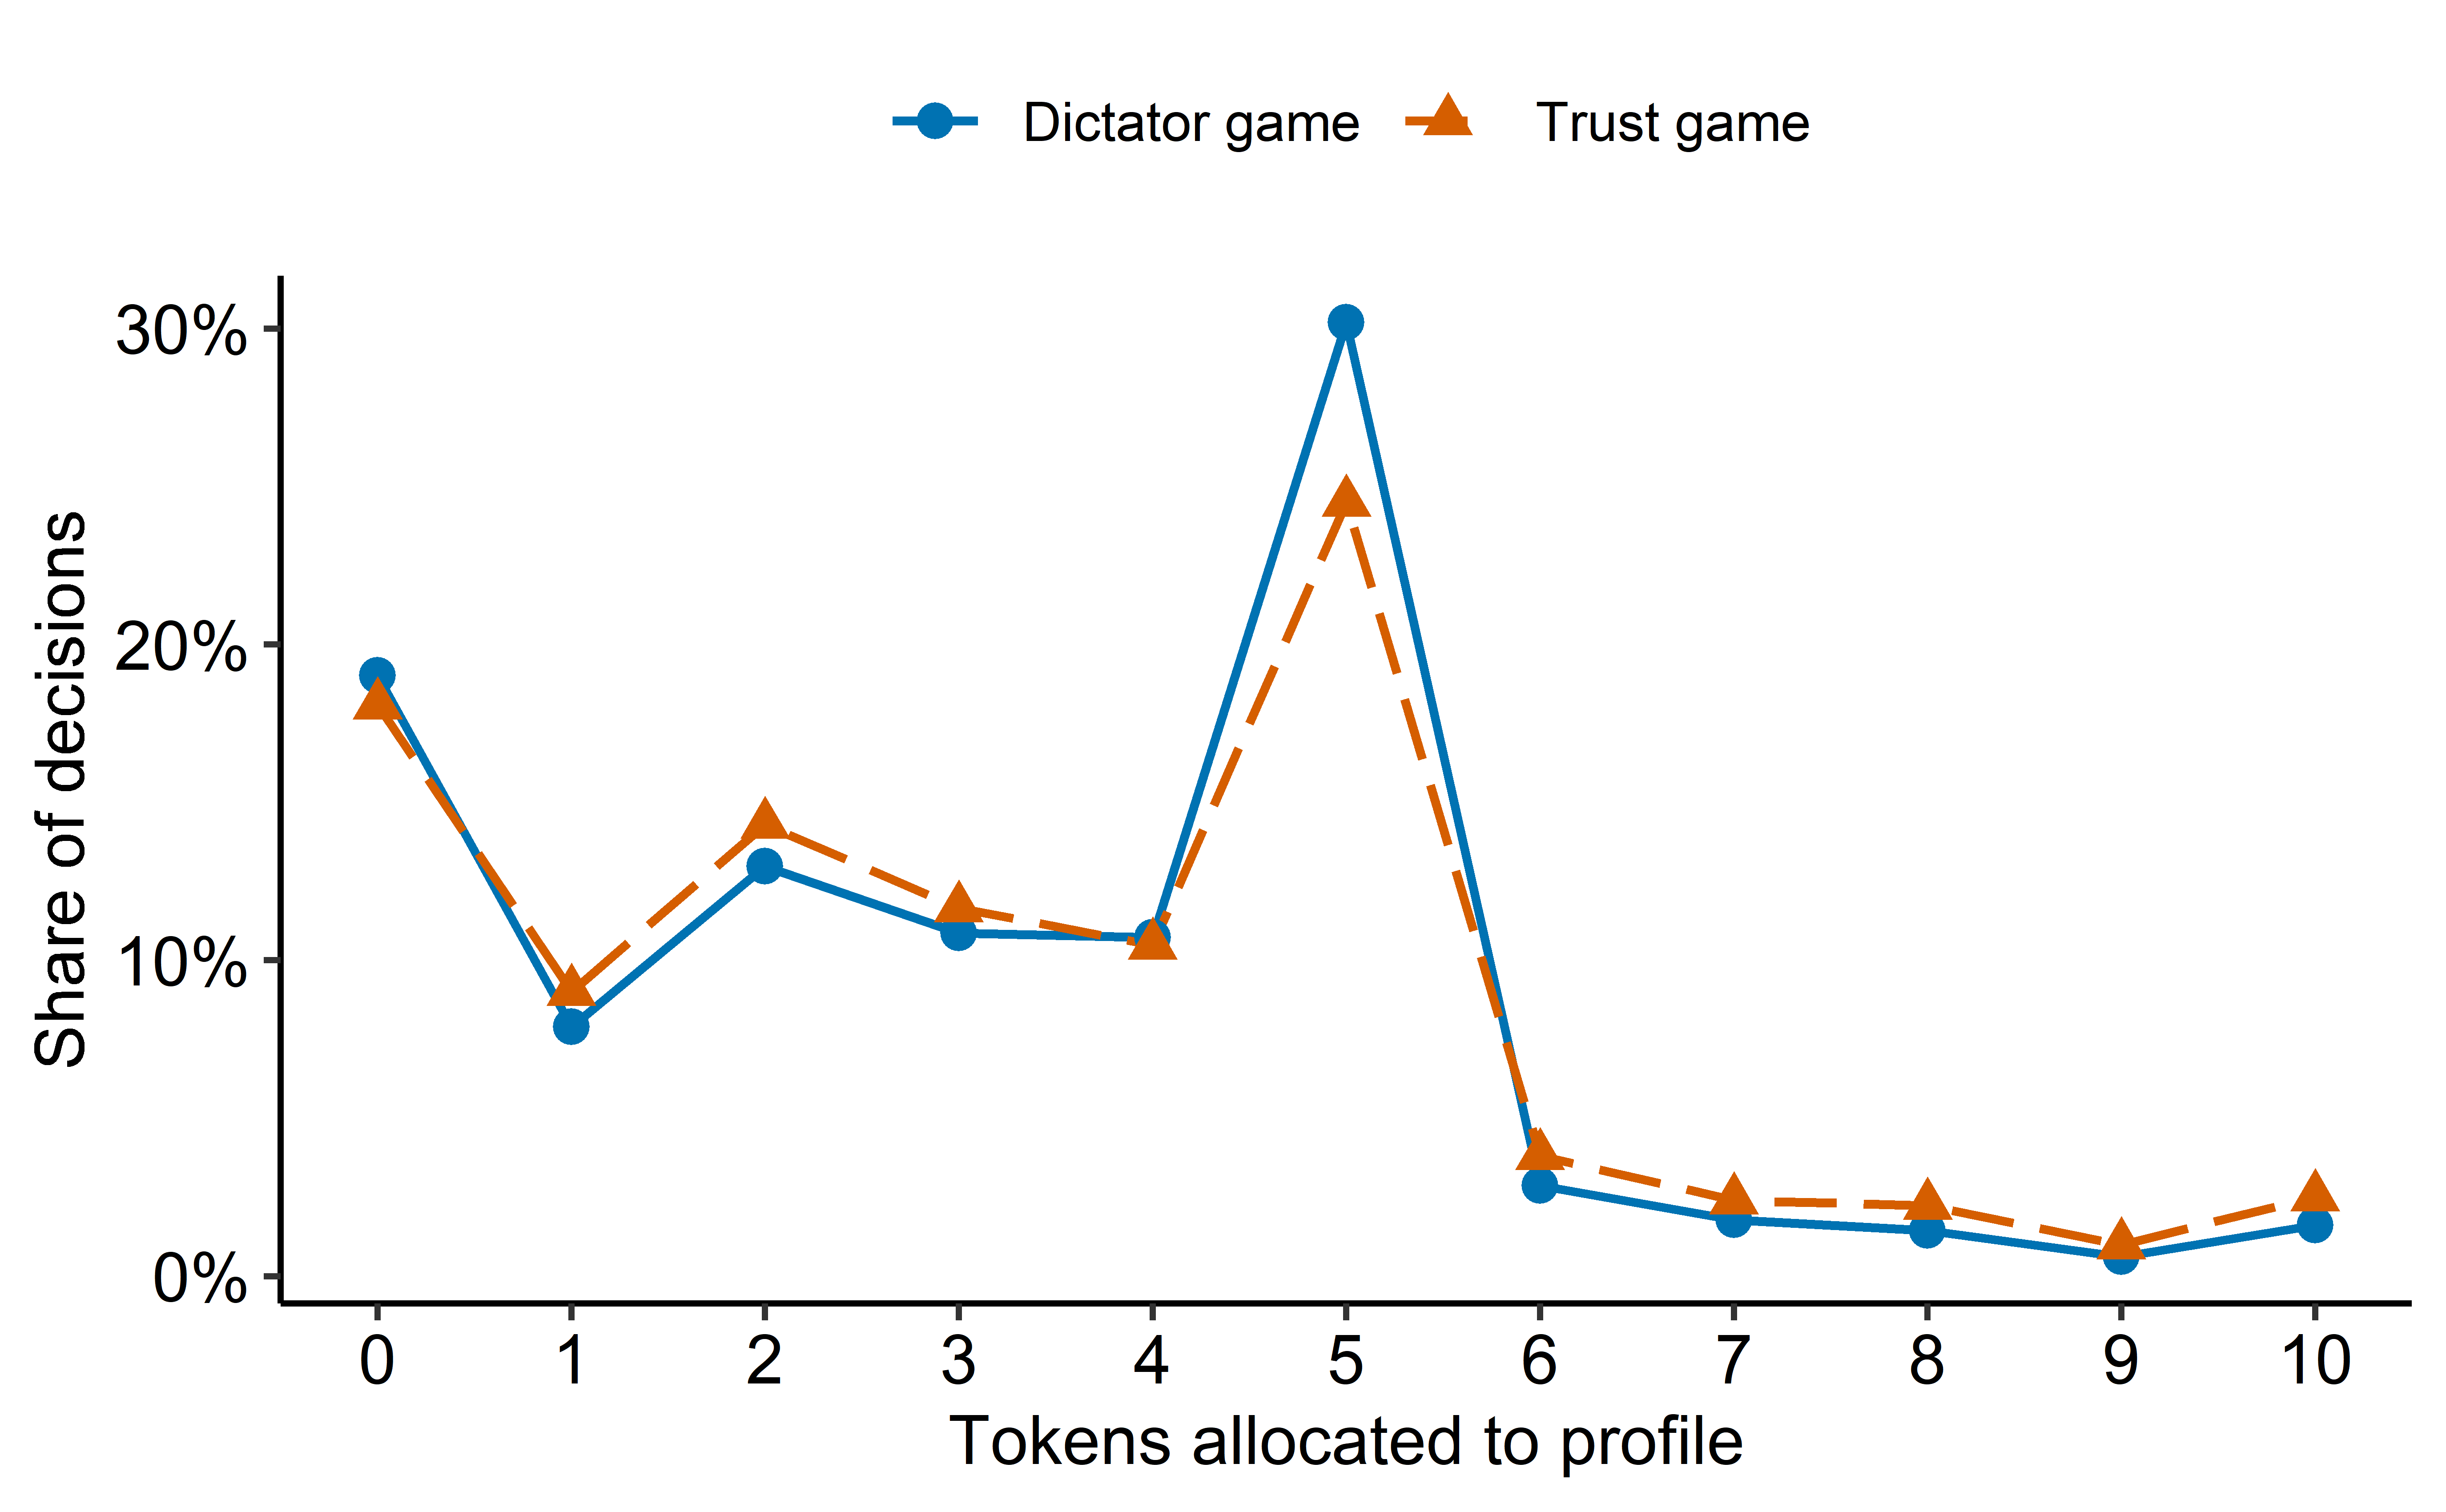
\includegraphics[keepaspectratio]{index_files/figure-latex/code-09_additional_figs_tables-fig-outcome-distr-output-1.png}}

}

\caption{\label{fig-outcome-distr}Distribution of outcomes (tokens
allocated to the displayed profile) by game. Points are the within-game
share of decisions at each integer token value, connected within game.
\(N=84.603\) in both games.}

\end{figure}%

\textsubscript{Source:
\href{https://dertristan.github.io/MBEU25/code/09_additional_figs_tables-preview.html\#cell-fig-outcome-distr}{Additional
Figures \& Tables}}

\subsubsection*{Distribution of Profile-level
Covariates}\label{distribution-of-profile-level-covariates}
\addcontentsline{toc}{subsubsection}{Distribution of Profile-level
Covariates}

{

\begin{longtable}[]{@{}
  >{\raggedright\arraybackslash}p{(\linewidth - 4\tabcolsep) * \real{0.2857}}
  >{\centering\arraybackslash}p{(\linewidth - 4\tabcolsep) * \real{0.3766}}
  >{\centering\arraybackslash}p{(\linewidth - 4\tabcolsep) * \real{0.3117}}@{}}

\caption{\label{tbl-balance-round-mods}Profile level covariates
distributions by treatment. Cells show raw counts with column
percentages in parentheses for categorical variables, and the median
with the first and third quartiles (Q1, Q3) in parentheses for numeric
variables.}

\tabularnewline

\toprule\noalign{}
\begin{minipage}[b]{\linewidth}\raggedright
\textbf{Variable}
\end{minipage} & \begin{minipage}[b]{\linewidth}\centering
\textbf{Non-Muslim} N = 126,663
\end{minipage} & \begin{minipage}[b]{\linewidth}\centering
\textbf{Muslim} N = 42,543
\end{minipage} \\
\midrule\noalign{}
\endhead
\bottomrule\noalign{}
\endlastfoot
cj\_nat & & \\
eu & 31,620 (25\%) & 10,483 (25\%) \\
non\_eu & 31,952 (25\%) & 10,548 (25\%) \\
own\_country & 63,091 (50\%) & 21,512 (51\%) \\
der\_cj\_eu\_identity & & \\
eu\_citizen & 34,470 (27\%) & 11,558 (27\%) \\
not\_displayed & 57,469 (45\%) & 19,544 (46\%) \\
not\_eu\_citizen & 34,724 (27\%) & 11,441 (27\%) \\
der\_cj\_partisanship & & \\
not\_applicable & 40,206 (32\%) & 13,560 (32\%) \\
not\_shown & 17,130 (14\%) & 5,874 (14\%) \\
shown & 69,327 (55\%) & 23,109 (54\%) \\
cj\_age & & \\
18 & 25,347 (20\%) & 8,539 (20\%) \\
30 & 25,348 (20\%) & 8,373 (20\%) \\
42 & 25,244 (20\%) & 8,611 (20\%) \\
53 & 25,521 (20\%) & 8,622 (20\%) \\
65 & 25,203 (20\%) & 8,398 (20\%) \\
cj\_sex & & \\
female & 63,308 (50\%) & 21,338 (50\%) \\
male & 63,355 (50\%) & 21,205 (50\%) \\
cj\_class & & \\
lower & 42,023 (33\%) & 14,048 (33\%) \\
middle & 42,393 (33\%) & 14,294 (34\%) \\
upper & 42,247 (33\%) & 14,201 (33\%) \\

\end{longtable}

}

\textsubscript{Source:
\href{https://dertristan.github.io/MBEU25/code/09_additional_figs_tables-preview.html\#cell-tbl-balance-round-mods}{Additional
Figures \& Tables}}

\subsubsection*{Distribution of Respondent-level
Covariates}\label{distribution-of-respondent-level-covariates}
\addcontentsline{toc}{subsubsection}{Distribution of Respondent-level
Covariates}

{

\begin{longtable}[]{@{}
  >{\raggedright\arraybackslash}p{(\linewidth - 4\tabcolsep) * \real{0.3462}}
  >{\raggedright\arraybackslash}p{(\linewidth - 4\tabcolsep) * \real{0.3462}}
  >{\raggedright\arraybackslash}p{(\linewidth - 4\tabcolsep) * \real{0.2821}}@{}}

\caption{\label{tbl-balance-resp-mods}Individual level covariate
distributions by treatment. Cells show raw counts with column
percentages in parentheses for categorical variables, and the median
with the first and third quartiles (Q1, Q3) in parentheses for numeric
variables.}

\tabularnewline

\toprule\noalign{}
\begin{minipage}[b]{\linewidth}\raggedright
\textbf{Variable}
\end{minipage} & \begin{minipage}[b]{\linewidth}\raggedright
\textbf{Non-Muslim} N = 16,622
\end{minipage} & \begin{minipage}[b]{\linewidth}\raggedright
\textbf{Muslim} N = 5,537
\end{minipage} \\
\midrule\noalign{}
\endhead
\bottomrule\noalign{}
\endlastfoot
q\_gender & & \\
female & 8,770 (53\%) & 2,985 (54\%) \\
male & 7,826 (47\%) & 2,548 (46\%) \\
other & 26 (0.2\%) & 4 (\textless0.1\%) \\
q\_age & 46 (34, 57) & 46 (34, 58) \\
q\_identity\_country & 1 (1, 2) & 1 (1, 2) \\
q\_identity\_eu & 3 (2, 4) & 3 (2, 4) \\
q\_identity\_europe & 2 (2, 3) & 2 (2, 3) \\
q\_religion & & \\
atheist & 1,996 (12\%) & 634 (11\%) \\
buddhist & 64 (0.4\%) & 20 (0.4\%) \\
catholic & 5,592 (34\%) & 1,911 (35\%) \\
dont\_know & 687 (4.1\%) & 209 (3.8\%) \\
hindu & 22 (0.1\%) & 2 (\textless0.1\%) \\
jewish & 37 (0.2\%) & 9 (0.2\%) \\
muslim & 80 (0.5\%) & 33 (0.6\%) \\
nonbeliever\_agnostic & 3,559 (21\%) & 1,214 (22\%) \\
orthodox & 1,823 (11\%) & 570 (10\%) \\
other & 589 (3.5\%) & 177 (3.2\%) \\
other\_christian & 729 (4.4\%) & 239 (4.3\%) \\
protestant & 1,439 (8.7\%) & 518 (9.4\%) \\
sikh & 5 (\textless0.1\%) & 1 (\textless0.1\%) \\
q\_class & & \\
dont\_know & 540 (3.2\%) & 210 (3.8\%) \\
higher\_class & 106 (0.6\%) & 35 (0.6\%) \\
lower\_middle\_class & 3,217 (19\%) & 1,088 (20\%) \\
middle\_class & 7,848 (47\%) & 2,537 (46\%) \\
other & 7 (\textless0.1\%) & 2 (\textless0.1\%) \\
upper\_middle\_class & 1,541 (9.3\%) & 551 (10.0\%) \\
working\_class & 3,363 (20\%) & 1,114 (20\%) \\
q\_eu\_efficacy\_understand & 5 (4, 6) & 5 (4, 6) \\
q\_pop\_reps & 6 (5, 7) & 6 (5, 7) \\
q\_pop\_goodevil & 4 (3, 5) & 4 (3, 5) \\
q\_pop\_compromise & 5 (4, 6) & 5 (4, 6) \\
q\_dem\_compromise & 5 (5, 6) & 5 (5, 6) \\
q\_dem\_listen & 6 (5, 7) & 6 (5, 7) \\
q\_tech\_experts & 5 (4, 6) & 5 (4, 6) \\
q\_tech\_leaders & 6 (5, 7) & 6 (5, 7) \\
q\_party\_harm & 5 (4, 6) & 5 (4, 6) \\
q\_people\_incompetent & 4 (3, 5) & 4 (3, 6) \\
q\_eu\_longterm & 5 (4, 6) & 5 (4, 6) \\
q\_eu\_responsive & 6 (5, 7) & 6 (5, 7) \\
q\_eu\_imp\_nat\_econ & 3 (2, 3) & 3 (2, 3) \\
q\_eu\_imp\_nat\_cul & 3 (2, 4) & 3 (2, 4) \\
q\_eu\_imp\_nat\_pol & 3 (2, 4) & 3 (2, 4) \\
q\_eu\_abolish & 5 (3, 6) & 5 (3, 6) \\
q\_eu\_satisfaction & 4 (3, 5) & 4 (3, 5) \\
q\_rural\_urban & & \\
large\_city & 6,320 (38\%) & 2,123 (38\%) \\
rural & 2,969 (18\%) & 1,042 (19\%) \\
small\_med\_town & 7,333 (44\%) & 2,372 (43\%) \\
q\_edu\_age\_stop & 21.0 (18.0, 24.0) & 21.0 (18.0, 24.0) \\

\end{longtable}

}

\textsubscript{Source:
\href{https://dertristan.github.io/MBEU25/code/09_additional_figs_tables-preview.html\#cell-tbl-balance-resp-mods}{Additional
Figures \& Tables}}

\subsubsection*{Question Wordings and
Scales}\label{question-wordings-and-scales}
\addcontentsline{toc}{subsubsection}{Question Wordings and Scales}

{

\begin{longtable}[]{@{}
  >{\raggedright\arraybackslash}p{(\linewidth - 4\tabcolsep) * \real{0.2685}}
  >{\raggedright\arraybackslash}p{(\linewidth - 4\tabcolsep) * \real{0.5833}}
  >{\raggedright\arraybackslash}p{(\linewidth - 4\tabcolsep) * \real{0.1296}}@{}}

\caption{\label{tbl-wordings}Question wordings and scales of
individual-level covariates used in the analysis.}

\tabularnewline

\toprule\noalign{}
\begin{minipage}[b]{\linewidth}\raggedright
Variable
\end{minipage} & \begin{minipage}[b]{\linewidth}\raggedright
Question wording
\end{minipage} & \begin{minipage}[b]{\linewidth}\raggedright
Scale coding
\end{minipage} \\
\midrule\noalign{}
\endhead
\bottomrule\noalign{}
\endlastfoot
\texttt{q\_gender} & Please indicate your gender. & Categorical \\
\texttt{q\_religion} & Do you consider yourself to be\ldots? &
Categorical \\
\texttt{q\_class} & Do you see yourself and your household belonging
to\ldots? & Categorical \\
\texttt{q\_rural\_urban} & Would you say you live in a\ldots? &
Categorical \\
\texttt{q\_identity\_country} & Please tell me how attached you feel
to\ldots{} - {[}SURVEY COUNTRY{]} & 1 (very attached) to 5 (not at all
attached) \\
\texttt{q\_identity\_eu} & Please tell me how attached you feel
to\ldots{} - The European Union (EU) & 1 (very attached) to 5 (not at
all attached) \\
\texttt{q\_identity\_europe} & Please tell me how attached you feel
to\ldots{} - Europe & 1 (very attached) to 5 (not at all attached) \\
\texttt{q\_eu\_efficacy\_understand} & Please tell me to what extent you
agree or disagree with each of the following statements. - I can
understand and evaluate important political questions about the EU & 1
(strongly disagree) to 7 (strongly agree) \\
\texttt{q\_pop\_reps} & Please indicate how much you agree with each of
the following statements. - Elected officials talk too much and take too
little action. & 1 (strongly disagree) to 7 (strongly agree) \\
\texttt{q\_pop\_goodevil} & Please indicate how much you agree with each
of the following statements. - Politics is ultimately a struggle between
good and evil. & 1 (strongly disagree) to 7 (strongly agree) \\
\texttt{q\_pop\_compromise} & Please indicate how much you agree with
each of the following statements. - What people call ``compromise'' in
politics is really just selling out on one's principles. & 1 (strongly
disagree) to 7 (strongly agree) \\
\texttt{q\_dem\_compromise} & Please indicate how much you agree with
each of the following statements. - In a democracy it is important to
make compromises among differing viewpoints. & 1 (strongly disagree) to
7 (strongly agree) \\
\texttt{q\_age} & How old are you? & Age in years \\
\texttt{q\_dem\_listen} & Please indicate how much you agree with each
of the following statements. - It is important to listen to the opinion
of other groups. & 1 (strongly disagree) to 7 (strongly agree) \\
\texttt{q\_tech\_experts} & Please indicate how much you agree with each
of the following statements. - Our country would run better if political
decisions were left up to experts instead of politicians and citizens. &
1 (strongly disagree) to 7 (strongly agree) \\
\texttt{q\_tech\_leaders} & Please indicate how much you agree with each
of the following statements. - The leaders of our country should be more
educated and skilled than ordinary citizens. & 1 (strongly disagree) to
7 (strongly agree) \\
\texttt{q\_party\_harm} & Please indicate how much you agree with each
of the following statements. - Political parties do more harm than good
to society & 1 (strongly disagree) to 7 (strongly agree) \\
\texttt{q\_people\_incompetent} & Please indicate how much you agree
with each of the following statements. - Ordinary people don't know what
policies are good for them. & 1 (strongly disagree) to 7 (strongly
agree) \\
\texttt{q\_eu\_longterm} & In thinking about the European Union (EU) and
its decisions more generally, some people argue that it should act upon
its long-term goals without pandering to the demand of the people. On
the other hand, others argue that the EU should listen to the demand of
people, rather than to act upon its long-term goals. When it comes to
the question of whether the EU should act upon its long-term goals or it
should listen to the demand of the people, what is your opinion? - The
EU should act upon its long-term goals & 1 (strongly disagree) to 7
(strongly agree) \\
\texttt{q\_eu\_responsive} & In thinking about the European Union (EU)
and its decisions more generally, some people argue that it should act
upon its long-term goals without pandering to the demand of the people.
On the other hand, others argue that the EU should listen to the demand
of people, rather than to act upon its long-term goals. When it comes to
the question of whether the EU should act upon its long-term goals or it
should listen to the demand of the people, what is your opinion? - The
EU should listen to the demand of the people & 1 (strongly disagree) to
7 (strongly agree) \\
\texttt{q\_eu\_imp\_nat\_econ} & Could you tell me whether you think
that the EU has a rather positive or rather negative effect on each of
the following domains? - UK economy & 1 (very positive) to 5 (very
negative) \\
\texttt{q\_eu\_imp\_nat\_cul} & Could you tell me whether you think that
the EU has a rather positive or rather negative effect on each of the
following domains? - Our culture and identity & 1 (very positive) to 5
(very negative) \\
\texttt{q\_eu\_imp\_nat\_pol} & Could you tell me whether you think that
the EU has a rather positive or rather negative effect on each of the
following domains? - UK's political status and influence & 1 (very
positive) to 5 (very negative) \\
\texttt{q\_eu\_abolish} & Please tell me to what extent you agree or
disagree with each of the following statements. - If the EU started
making a lot of decisions that most people disagreed with, it might be
better to do away with the EU altogether & 1 (strongly disagree) to 7
(strongly agree) \\
\texttt{q\_eu\_satisfaction} & Please tell me to what extent you agree
or disagree with each of the following statements. - I am satisfied with
the performance of the EU & 1 (strongly disagree) to 7 (strongly
agree) \\
\texttt{q\_edu\_age\_stop} & How old were you when you stopped full-time
education? & Years \\

\end{longtable}

}

\textsubscript{Source:
\href{https://dertristan.github.io/MBEU25/code/09_additional_figs_tables-preview.html\#cell-tbl-wordings}{Additional
Figures \& Tables}}

\subsection*{Appendix B: Additional CF
Figures}\label{appendix-b-additional-cf-figures}
\addcontentsline{toc}{subsection}{Appendix B: Additional CF Figures}

\subsubsection*{TOC / AUTOC Curve}\label{toc-autoc-curve}
\addcontentsline{toc}{subsubsection}{TOC / AUTOC Curve}

\begin{figure}[H]

\centering{

\pandocbounded{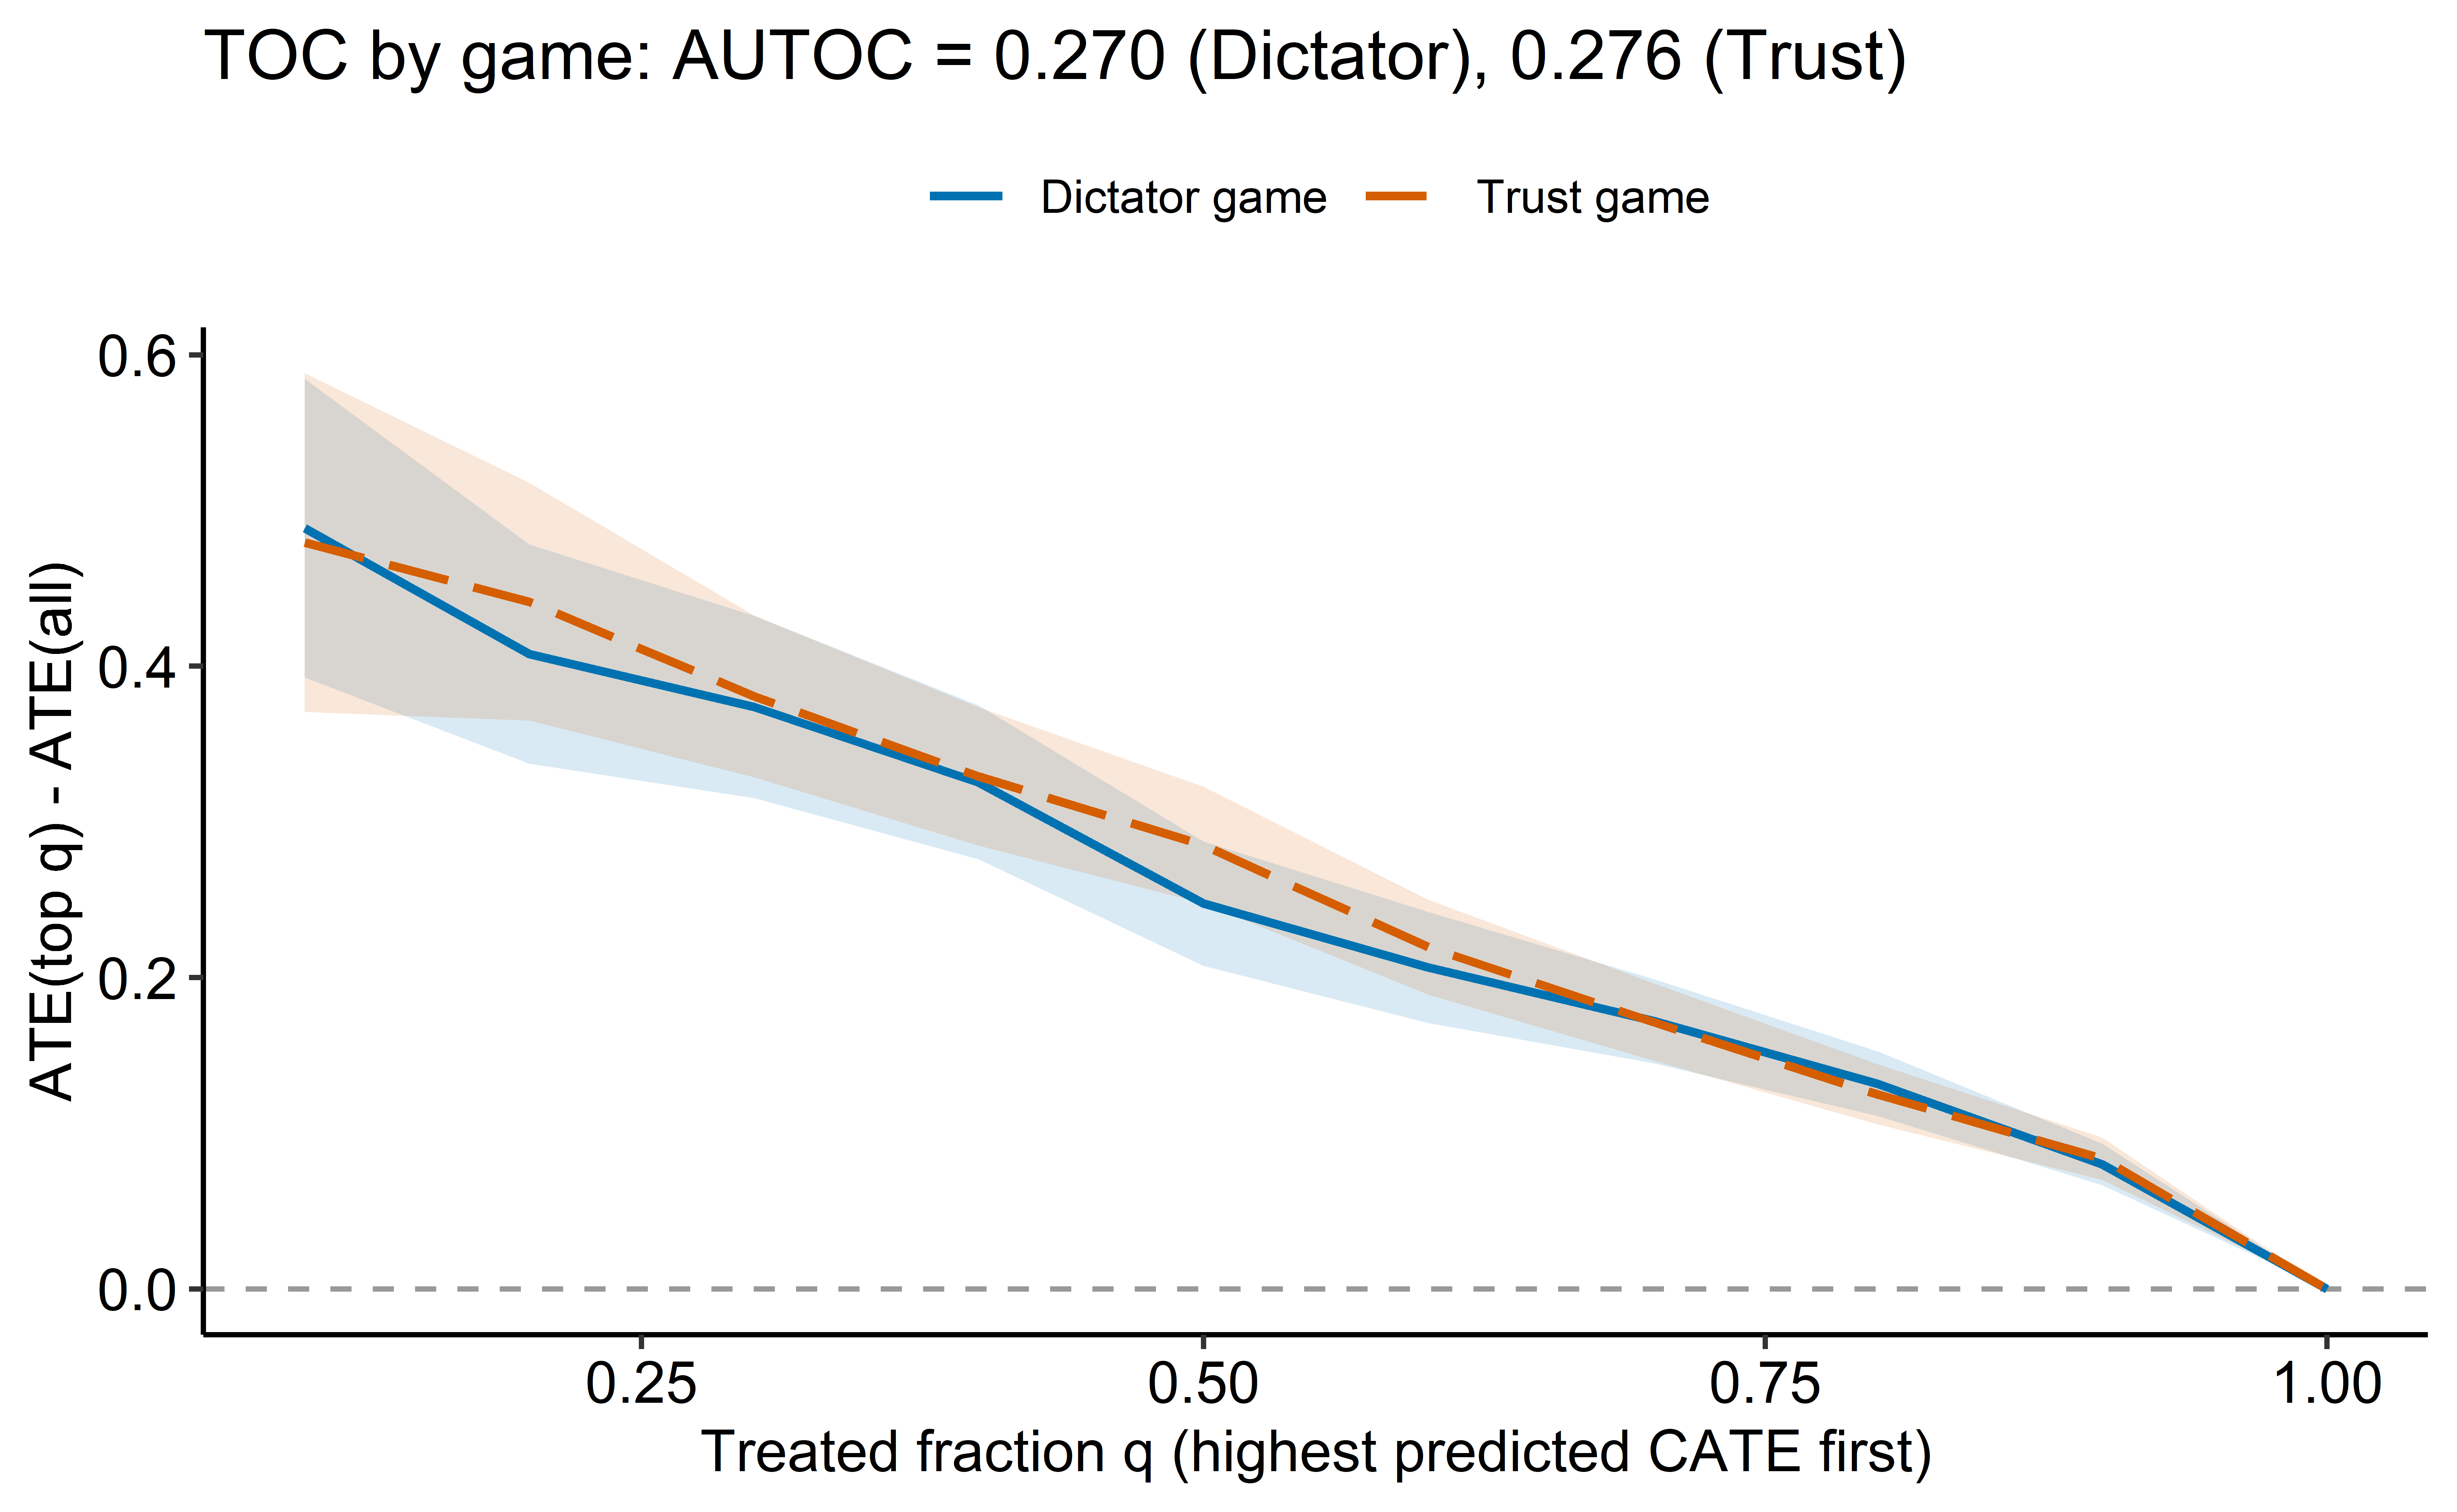
\includegraphics[keepaspectratio]{index_files/figure-latex/code-07_postprocess_grf-fig-grf-combined-toc-output-1.png}}

}

\caption{\label{fig-grf-combined-toc}CF Targeting Operator
Characteristic curve, both games overlaid: ATE among the top-q fraction
by predicted CATE minus the overall ATE, with 95\% CI ribbon. The area
under each curve is the AUTOC, reported in the title.}

\end{figure}%

\textsubscript{Source:
\href{https://dertristan.github.io/MBEU25/code/07_postprocess_grf-preview.html\#cell-fig-grf-combined-toc}{GRF
Post-Processing}}

\subsubsection*{Variable Importance}\label{variable-importance}
\addcontentsline{toc}{subsubsection}{Variable Importance}

\begin{figure}[H]

\centering{

\pandocbounded{\includegraphics[keepaspectratio]{index_files/figure-latex/code-07_postprocess_grf-fig-grf-combined-vi-output-1.png}}

}

\caption{\label{fig-grf-combined-vi}CF variable importance aggregated to
the original moderators, both games overlaid (dodged bars by game).
Profile-level and respondent-level moderators are separated into facets.
Within each facet moderators are ordered by their mean importance across
the two games. Country fixed-effect columns excluded.}

\end{figure}%

\textsubscript{Source:
\href{https://dertristan.github.io/MBEU25/code/07_postprocess_grf-preview.html\#cell-fig-grf-combined-vi}{GRF
Post-Processing}}

\subsection*{Appendix C: Main Results from BCF
Method}\label{appendix-c-main-results-from-bcf-method}
\addcontentsline{toc}{subsection}{Appendix C: Main Results from BCF
Method}

\subsubsection*{BCF Moderation by Profile-level
Covariates}\label{bcf-moderation-by-profile-level-covariates}
\addcontentsline{toc}{subsubsection}{BCF Moderation by Profile-level
Covariates}

\begin{figure}[H]

\centering{

\pandocbounded{\includegraphics[keepaspectratio]{index_files/figure-latex/code-08_postprocess_bcf-fig-bcf-combined-prof-output-1.png}}

}

\caption{\label{fig-bcf-combined-prof}BCF posterior estimates of the
profile-level CATE (\(\hat{\tau}_{ric}\)) of the Muslim profile across
the levels of every conjoint-round moderator (x-axis), Dictator and
Trust games overlaid and distinguished jointly by colour, shape, and
linetype. The y-axis is \(\hat{\tau}_{ric}\) on the token-allocation
scale. Each point is a per-level posterior median with a cluster-robust
95\% interval, formed as the median plus or minus 1.96 times a combined
standard error (a normal approximation) that adds the posterior SD of
the within-level mean to a respondent cluster-bootstrap SD. Grey bars
along the bottom of each facet show the per-level row count (pooled over
games). The y-axis is free per facet. In the Profile partisanship facet,
partisanship not shown refers to within the co-national category only,
since partisanship is displayed for co-national profiles only.}

\end{figure}%

\textsubscript{Source:
\href{https://dertristan.github.io/MBEU25/code/08_postprocess_bcf-preview.html\#cell-fig-bcf-combined-prof}{BCF
Post-Processing}}

\subsubsection*{BCF Moderation by Respondent-level
Covariates}\label{bcf-moderation-by-respondent-level-covariates}
\addcontentsline{toc}{subsubsection}{BCF Moderation by Respondent-level
Covariates}

\begin{figure}[H]

\centering{

\pandocbounded{\includegraphics[keepaspectratio]{index_files/figure-latex/code-08_postprocess_bcf-fig-bcf-combined-resp-1-output-1.png}}

}

\caption{\label{fig-bcf-combined-resp-1}BCF posterior estimates of the
respondent-level CATE (\(\hat{\tau}_i\)) of the Muslim profile across
the levels of the first half of the discrete individual-level moderators
(top panel) and across age (q\_age, bottom panel), Dictator and Trust
games overlaid and distinguished jointly by colour, shape, and linetype.
The y-axis is \(\hat{\tau}_i\) on the token-allocation scale. All item
scales are oriented so that higher x-axis values mean more agreement, a
more positive evaluation, or more attachment, depending on the item (see
Table~\ref{tbl-wordings}). Every point and ribbon value is a posterior
median with a cluster-robust 95\% interval, formed as the median plus or
minus 1.96 times a combined standard error (a normal approximation) that
adds the posterior SD to a respondent cluster-bootstrap SD. Top: ordered
numeric scales are drawn as a connecting line and interval ribbon per
game, categorical moderators as dodged points and intervals. Grey bars
show the per-level row count (pooled over games). Bottom: per-grid-cell
estimate, interval ribbon, and connecting line per game over a grey
histogram of the covariate, on 100 equal intervals across the full 18-75
years. The y-axis is free per facet. Discrete levels comprising less
than 1\% of a game's sample are dropped because their CATE is too
imprecise to compare.}

\end{figure}%

\textsubscript{Source:
\href{https://dertristan.github.io/MBEU25/code/08_postprocess_bcf-preview.html\#cell-fig-bcf-combined-resp-1}{BCF
Post-Processing}}

\begin{figure}[H]

\centering{

\pandocbounded{\includegraphics[keepaspectratio]{index_files/figure-latex/code-08_postprocess_bcf-fig-bcf-combined-resp-2-output-1.png}}

}

\caption{\label{fig-bcf-combined-resp-2}BCF posterior estimates of the
respondent-level CATE (\(\hat{\tau}_i\)) of the Muslim profile across
the levels of the second half of the discrete individual-level
moderators (top panel) and across age at which education stopped
(q\_edu\_age\_stop, bottom panel), Dictator and Trust games overlaid and
distinguished jointly by colour, shape, and linetype. The y-axis is
\(\hat{\tau}_i\) on the token-allocation scale. All item scales are
oriented so that higher x-axis values mean more agreement, a more
positive evaluation, or more attachment, depending on the item (see
Table~\ref{tbl-wordings}). Every ribbon value is a posterior median with
a cluster-robust 95\% interval, formed as the median plus or minus 1.96
times a combined standard error (a normal approximation) that adds the
posterior SD to a respondent cluster-bootstrap SD. Top: ordered numeric
scales are drawn as a connecting line and interval ribbon per game. Grey
bars show the per-level row count (pooled over games). Bottom: per-year
posterior median, interval ribbon, and connecting line per game at each
integer year of education-stopping age from 15 to 30, over a grey
histogram of the covariate. The y-axis is free per facet. Discrete
levels comprising less than 1\% of a game's sample are dropped because
their CATE is too imprecise to compare.}

\end{figure}%

\textsubscript{Source:
\href{https://dertristan.github.io/MBEU25/code/08_postprocess_bcf-preview.html\#cell-fig-bcf-combined-resp-2}{BCF
Post-Processing}}




\end{document}
